\section{Quantità di vegetazione in alveo}
Si è quantificato l'areale delle isole presenti in alveo avendo accortezza di distinguerlo chiaramente dall'areale della \emph{floodplain}, il quale è soggetto a dinamiche diverse rispetto alle isole.

\subsection{Metodi: classificare l'alveo}
Per classificare il terreno occupato dall'alveo è stato seguito l'approccio di altri autori in analisi simili eseguite su immagini \AST{} e LandSat~TM \squarecites{Bertoldi:2011-ASTER}{Henshaw:2013-LandSat}.
%
\begin{description}
	\item[Maschera computazionale] 
	Dapprima è stata individuata manualmente una maschera di calcolo che comprendesse l'alveo attivo e la parte di piana alluvionale che è stata erosa quando coinvolta nelle piene; 
	tale maschera si estende da Tolmezzo al ponte di Madrisio
	(\vref{fig:esempio-maschera}). 
	Applicandola, il dominio computazionale è stato ridotto a comprendere l'inviluppo degli alvei attivi che si sono succeduti dall'immagine del~2000 a quella del~2018.
	%
	\begin{figure}[t]
		\centering
		\begin{subfigure}[b]{0.296\textwidth}
			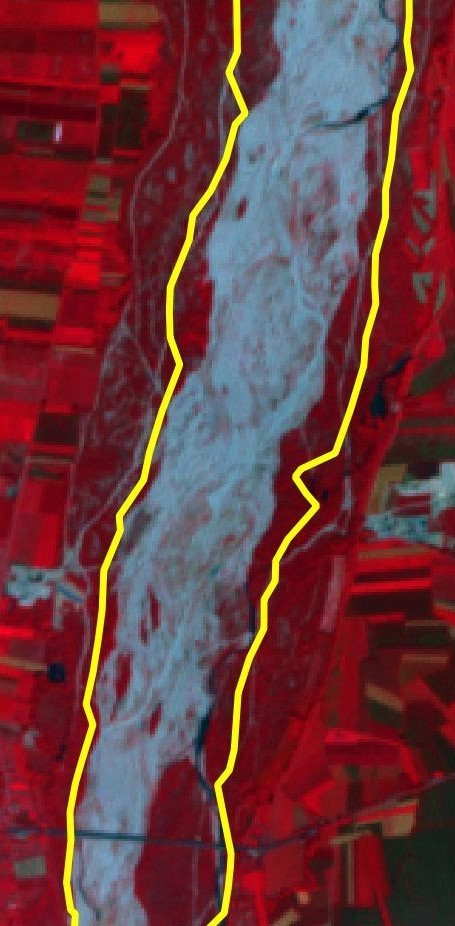
\includegraphics[width=\textwidth]{files/esempio_mask_2000_09_17.jpeg}
			\caption{\AST{} 2000-09-17.}
		\end{subfigure}
		\qquad
		\begin{subfigure}[b]{0.30\textwidth}
			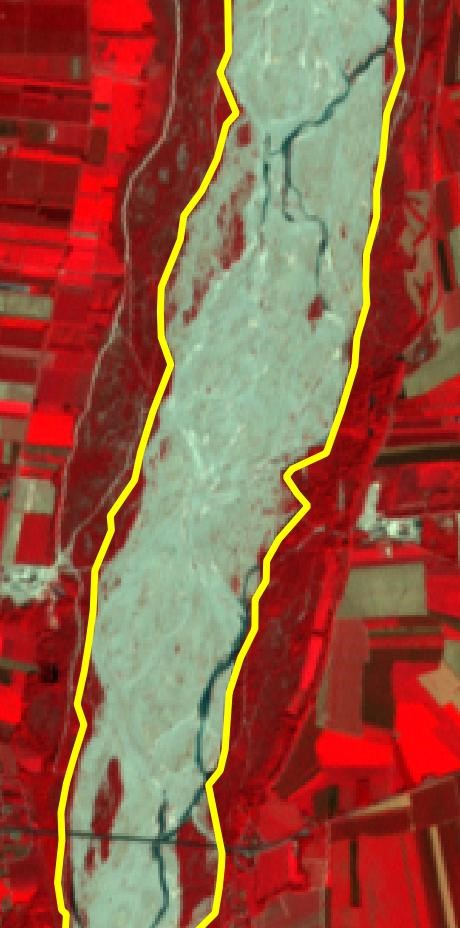
\includegraphics[width=\textwidth]{files/esempio_mask_2015_09_11.jpeg}
			\caption{\AST{} 2015-09-11.}
		\end{subfigure}
		\caption[definizione della maschera per limitare il dominio computazionale]
			{esempio in cui si vede come la maschera utilizzata per limitare il dominio computazionale (in giallo) sia il risultato dell'inviluppo degli alvei attivi che si sono modificati nel tempo; le immagini sono in falsi colori (IR-R-G).}
		\label{fig:esempio-maschera}
	\end{figure}
	%
	%
	\item[NDVI] 
	In questa area è stato calcolato il \emph{Normalized Difference Vegetation Index} (NDVI) grazie alle bande del \emph{Near Infrared} (NIR) e del \emph{Red} (R)
	%
	\begin{equation}
		%\notag
		NDVI = \frac{NIR - R}{NIR + R} \quad .
		\label{eq:ndvi}
	\end{equation}
	%
	%
	\item[Aree campione]
	\`{E} stata effettuata una digitalizzazione manuale di alcune aree campione per le immagini \AST{} del~2005-08-30 ($\sim 70$) e del~2012-08-01 ($\sim 100$), le immagini Plaiades del~2014-10-31 ($\sim 40$) e del~2015-06-13 ($\sim 40$), l'immagine \Se{} del~2017-04-21 ($\sim 45$) e l'immagine \WV{} del 2018-06-15 ($\sim 55$) (\vref{fig:esempio-aree-campione}).
	Sono state selezionate immagini per ogni satellite poiché ciascuno è sensibile a bande leggermente diverse. 
	%; si sono osservate due immagini \AST{} dato il grande numero di immagini disponibili da questo sensore scegliendo quelle con minor nuvolosità.
	\\
	Queste aree campione sono state suddivise in tre classi: vegetazione, alveo attivo e canale.
	%
	\begin{figure}[ht]
		\centering
		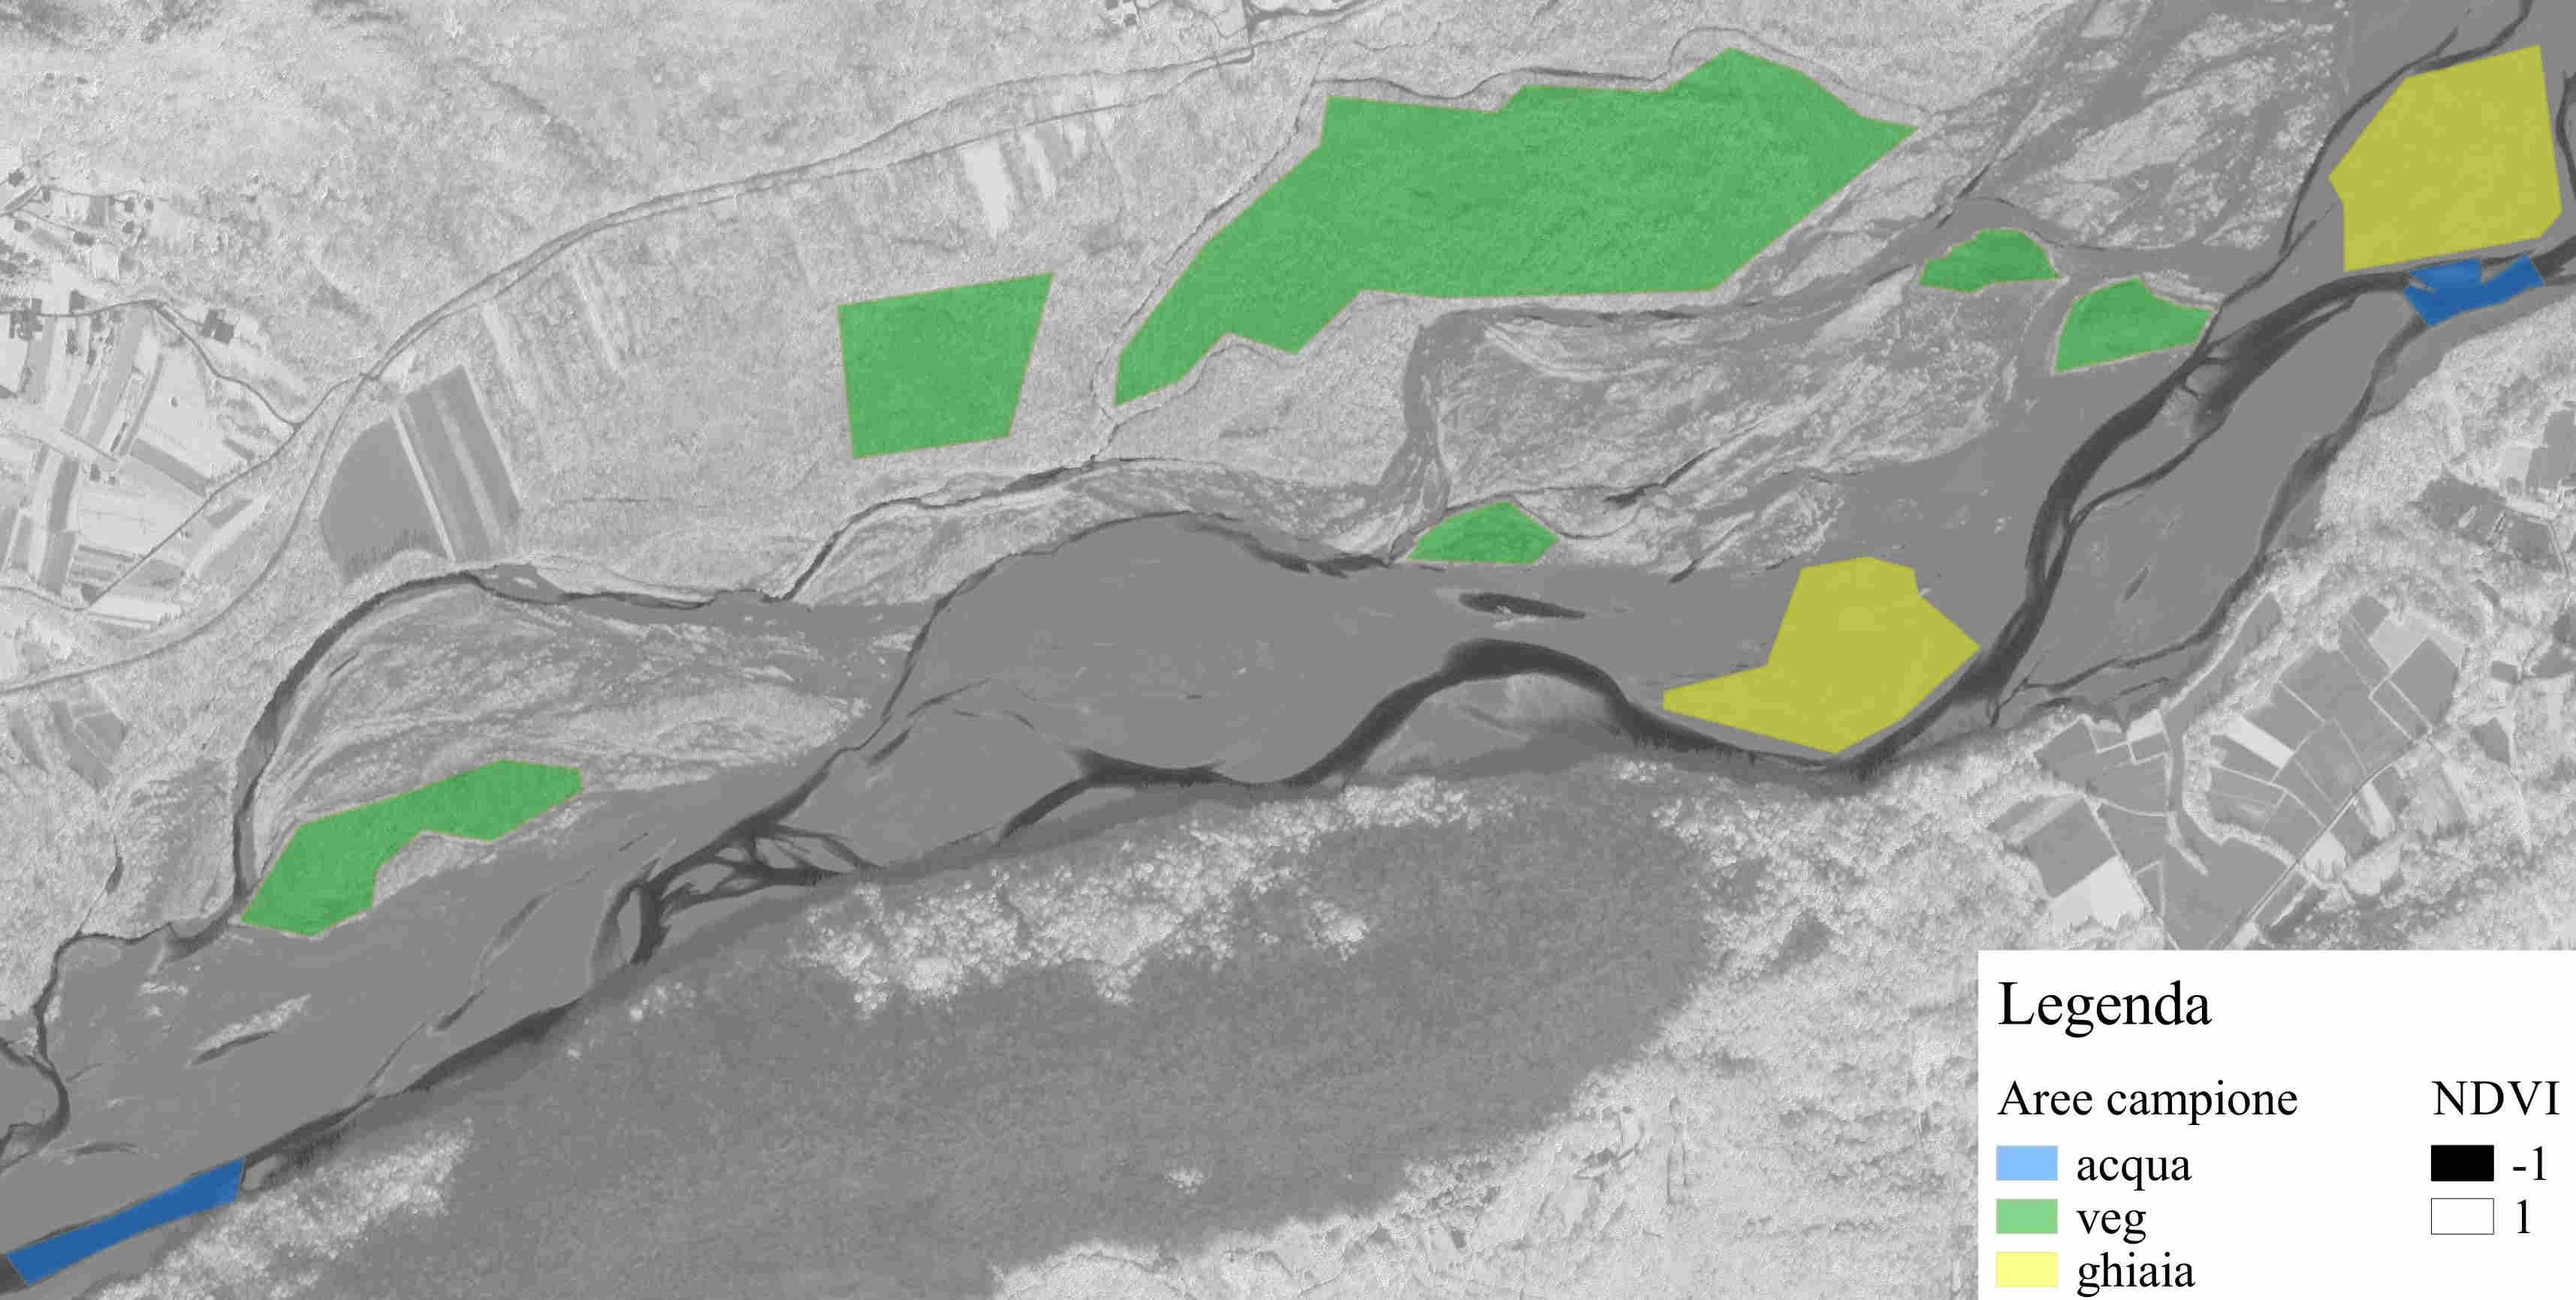
\includegraphics[width=\textwidth]{files/esempio_aree_campione_2014_10_31.jpeg}
		\caption[esempio di aree campione per calcolare la distribuzione dell'NDVI]{esempio di digitalizzazione di alcune aree campione per l'immagine \Pl{} del~2014-10-31; sullo sfondo la mappa dell'NDVI.}
		\label{fig:esempio-aree-campione}
	\end{figure}
	%
	%
	\item[Percentili aree campione]
	Per ogni immagine si è osservata la distribuzione dell'NDVI in ogni classe (\vref{graph:percentili}).
	% 
	\begin{figure}[ht]
		\centering
		\begin{tikzpicture}
	\begin{groupplot}[
		group style = {
			group size = 2 by 3,
			ylabels at = edge left,
			x descriptions at = edge bottom,
			horizontal sep = 1.1cm,
			vertical sep = 0.1cm,
		},
		width = 0.45\textwidth,
		height = 0.45\textwidth,
		ylabel = NDVI,
		boxplot/draw direction = y,
		xtick = {1,2,3},
		xticklabels = {Veg., Alveo, Canale},
		ymax = 0.795,
		ymin = -0.50,
		grid = major,
	]
	\nextgroupplot % ASTER 2005-08-31
		\addplot+ [ % vegetazione
			teal, very thick,
			boxplot prepared = {
				lower whisker = 0.353656,
				lower quartile = 0.470411,
				median = 0.560063,
				upper quartile = 0.614701,
				upper whisker = 0.644957,
				},
        	]
        	coordinates {};
		\addplot+ [ % alveo attivo
			brown, very thick,
			boxplot prepared = {
				lower whisker = 0.077472,
				lower quartile = 0.091653,
				median = 0.122488,
				upper quartile = 0.149573,
				upper whisker = 0.171459,
				},
        	]
        	coordinates {};
		\addplot+ [ % canale
			cyan, very thick,
			boxplot prepared = {
				lower whisker = -0.477885,
				lower quartile = -0.362798,
				median = -0.269905,
				upper quartile = -0.058787,
				upper whisker = 0.072414,
				},
        	]
        	coordinates {};
        \node [fill = white, draw = black, anchor = north east] 
        	at (axis description cs: 1,1) {AST 2005-08-31};
	%------------------------------------------------------
	\nextgroupplot % ASTER 2012-08-01
		\addplot+ [ % vegetazione
			teal, very thick,
			boxplot prepared = {
				lower whisker = 0.341613,
				lower quartile = 0.444200,
				median = 0.586294,
				upper quartile = 0.672889,
				upper whisker = 0.709027,
				},
        	]
        	coordinates {};
		\addplot+ [ % alveo attivo
			brown, very thick,
			boxplot prepared = {
				lower whisker = 0.10506,
				lower quartile = 0.117969,
				median = 0.143631,
				upper quartile = 0.16549,
				upper whisker = 0.184871,
				},
        	]
        	coordinates {};
		\addplot+ [ % canale
			cyan, very thick,
			boxplot prepared = {
				lower whisker = -0.432201,
				lower quartile = -0.379825,
				median = -0.322239,
				upper quartile = -0.226459,
				upper whisker = -0.103914,
				},
        	]
        	coordinates {};
        \node [fill = white, draw = black, anchor = north east] 
        	at (axis description cs: 1,1) {AST 2012-08-01};
	%------------------------------------------------------
	\nextgroupplot % Pleiades 2014-10-31
		\addplot+ [ % vegetazione
			teal, very thick,
			boxplot prepared = {
				lower whisker = 0.286467,
				lower quartile = 0.350238,
				median = 0.415502,
				upper quartile = 0.483495,
				upper whisker = 0.549505,
				},
        	]
        	coordinates {};
		\addplot+ [ % alveo attivo
			brown, very thick,
			boxplot prepared = {
				lower whisker = 0.049796,
				lower quartile = 0.055794,
				median = 0.063049,
				upper quartile = 0.07173,
				upper whisker = 0.081427,
				},
        	]
        	coordinates {};
		\addplot+ [ % canale
			cyan, very thick,
			boxplot prepared = {
				lower whisker = -0.426415,
				lower quartile = -0.387978,
				median = -0.338308,
				upper quartile = -0.266515,
				upper whisker = -0.175373,
				},
        	]
        	coordinates {};
        \node [fill = white, draw = black, anchor = north east] 
        	at (axis description cs: 1,1) {PL 2014-10-31};
	%------------------------------------------------------
	\nextgroupplot % Pleiades 2015-08-13
		\addplot+ [ % vegetazione
			teal, very thick,
			boxplot prepared = {
				lower whisker = 0.415693,
				lower quartile = 0.5,
				median = 0.570359,
				upper quartile = 0.638507,
				upper whisker = 0.704044		
,
				},
        	]
        	coordinates {};
		\addplot+ [ % alveo attivo
			brown, very thick,
			boxplot prepared = {
				lower whisker = 0.075052,
				lower quartile = 0.080858,
				median = 0.087921,
				upper quartile = 0.096031,
				upper whisker = 0.106198,
				},
        	]
        	coordinates {};
		\addplot+ [ % canale
			cyan, very thick,
			boxplot prepared = {
				lower whisker = -0.262599,
				lower quartile = -0.244228,
				median = -0.214393,
				upper quartile = -0.176471,
				upper whisker = -0.132762,
				},
        	]
        	coordinates {};
        \node [fill = white, draw = black, anchor = north east] 
        	at (axis description cs: 1,1) {PL 2015-08-13};
	%------------------------------------------------------
	\nextgroupplot % Sentinel2 2017-04-21
		\addplot+ [ % vegetazione
			teal, very thick,
			boxplot prepared = {
				lower whisker = 0.163722,
				lower quartile = 0.241916,
				median = 0.374344,
				upper quartile = 0.548241,
				upper whisker = 0.672782,
				},
        	]
        	coordinates {};
		\addplot+ [ % alveo attivo
			brown, very thick,
			boxplot prepared = {
				lower whisker = 0.056176,
				lower quartile = 0.061278,
				median = 0.067681,
				upper quartile = 0.076396,
				upper whisker = 0.089304,
				},
        	]
        	coordinates {};
		\addplot+ [ % canale
			cyan, very thick,
			boxplot prepared = {
				lower whisker = -0.322237,
				lower quartile = -0.288822,
				median = -0.239533,
				upper quartile = -0.177094,
				upper whisker = -0.131119,
				},
        	]
        	coordinates {};
        \node [fill = white, draw = black, anchor = north east] 
        	at (axis description cs: 1,1) {S2 2017-04-21};
	%------------------------------------------------------
	\nextgroupplot % WorldView2 2018-06-15
		\addplot+ [ % vegetazione
			teal, very thick,
			boxplot prepared = {
				lower whisker = 0.569665,
				lower quartile = 0.657917,
				median = 0.719523,
				upper quartile = 0.759148,
				upper whisker = 0.791594,
				},
        	]
        	coordinates {};
		\addplot+ [ % alveo attivo
			brown, very thick,
			boxplot prepared = {
				lower whisker = 0.126214,
				lower quartile = 0.129661,
				median = 0.13373,
				upper quartile = 0.138542,
				upper whisker = 0.149326,
				},
        	]
        	coordinates {};
		\addplot+ [ % canale
			cyan, very thick,
			boxplot prepared = {
				lower whisker = -0.416974,
				lower quartile = -0.392405,
				median = -0.365385,
				upper quartile = -0.335135,
				upper whisker = -0.29979,
				},
        	]
        	coordinates {};
        \node [fill = white, draw = black, anchor = north east] 
        	at (axis description cs: 1,1) {WV2 2018-06-15};
	\end{groupplot}
\end{tikzpicture}

		\caption[boxplot dell'NDVI nelle aree campione in quattro immagini satellitari]{boxplot dell'NDVI nelle aree campione in quattro immagini satellitari; i baffi indicano il 10mo e il 90mo percentile, gli estremi della scatola rappresentano il 25mo e il 75mo percentile, la linea nella scatola è la mediana.}
		\label{graph:percentili}
	\end{figure}
	%
	%
	\item[Soglie NDVI] 
	Da tali grafici sono state ottenute delle soglie di NDVI per classificare le immagini satellitari (\vref{tab:ndvi-soglia}); per l'immagine \WV{} la soglia che distingue vegetazione da alveo attivo è maggiore. Le soglie sono in accordo con quanto riportato in letteratura \squarecite{Bertoldi:2011-ASTER}.
	%
	\begin{table}[ht]
		\centering
		\begin{tabular}{
			c 
			S[table-format=1.1]@{\,}
			c@{\,}
			c@{\,}
			c@{\,}
			S[table-format=1.1]
			S[table-format=1.1]@{\,}
			c@{\,}
			c@{\,}
			c@{\,}
			S[table-format=1.1]
			}
			\toprule
			&	\multicolumn{5}{c}{\textbf{Soglie AST PL S2}}	&	\multicolumn{5}{c}{\textbf{Soglie WV2}}	\\
			\midrule
			Vegetazione		&	0.2	&	$\leq$	&	NDVI	&			&		& 	0.3	&	$\leq$	&	NDVI	&			& 	\\
			Alveo attivo	&	0.0	&	$\leq$	&	NDVI	&	$<$		&	0.2	&	0.0	&	$\leq$	&	NDVI	&	$<$		&	0.3\\
			Canale			&		&			&	NDVI	&	$<$		&	0.0	&		&			&	NDVI	&	$<$		&	0.0\\
			\bottomrule
		\end{tabular}
		\caption[soglie NDVI]{soglie di NDVI per la classificazione delle immagini satellitari.}
		\label{tab:ndvi-soglia}
	\end{table}
	%
	%
	\item[Divisione in 23 tratti]
	La maschera di calcolo è stata suddivisa manualmente in 23~tratti con 22~sezioni al fine di avere un maggior dettaglio spaziale delle dinamiche di vegetazione (\vref{fig:23-tratti}). 
	Questi tratti sono stati selezionati in modo da possedere caratteristiche omogenee per portata e crescita della vegetazione; 
	pertanto confluenze di immissari, bruschi restringimenti o allargamenti, inizio di pronunciato \emph{upwelling} o \emph{downwelling} ed evidenti cambiamenti di morfologia fluviale sono stati gli elementi per individuare le 22~sezioni che determinano i 23~tratti.
	%
	\begin{figure}
		\centering
		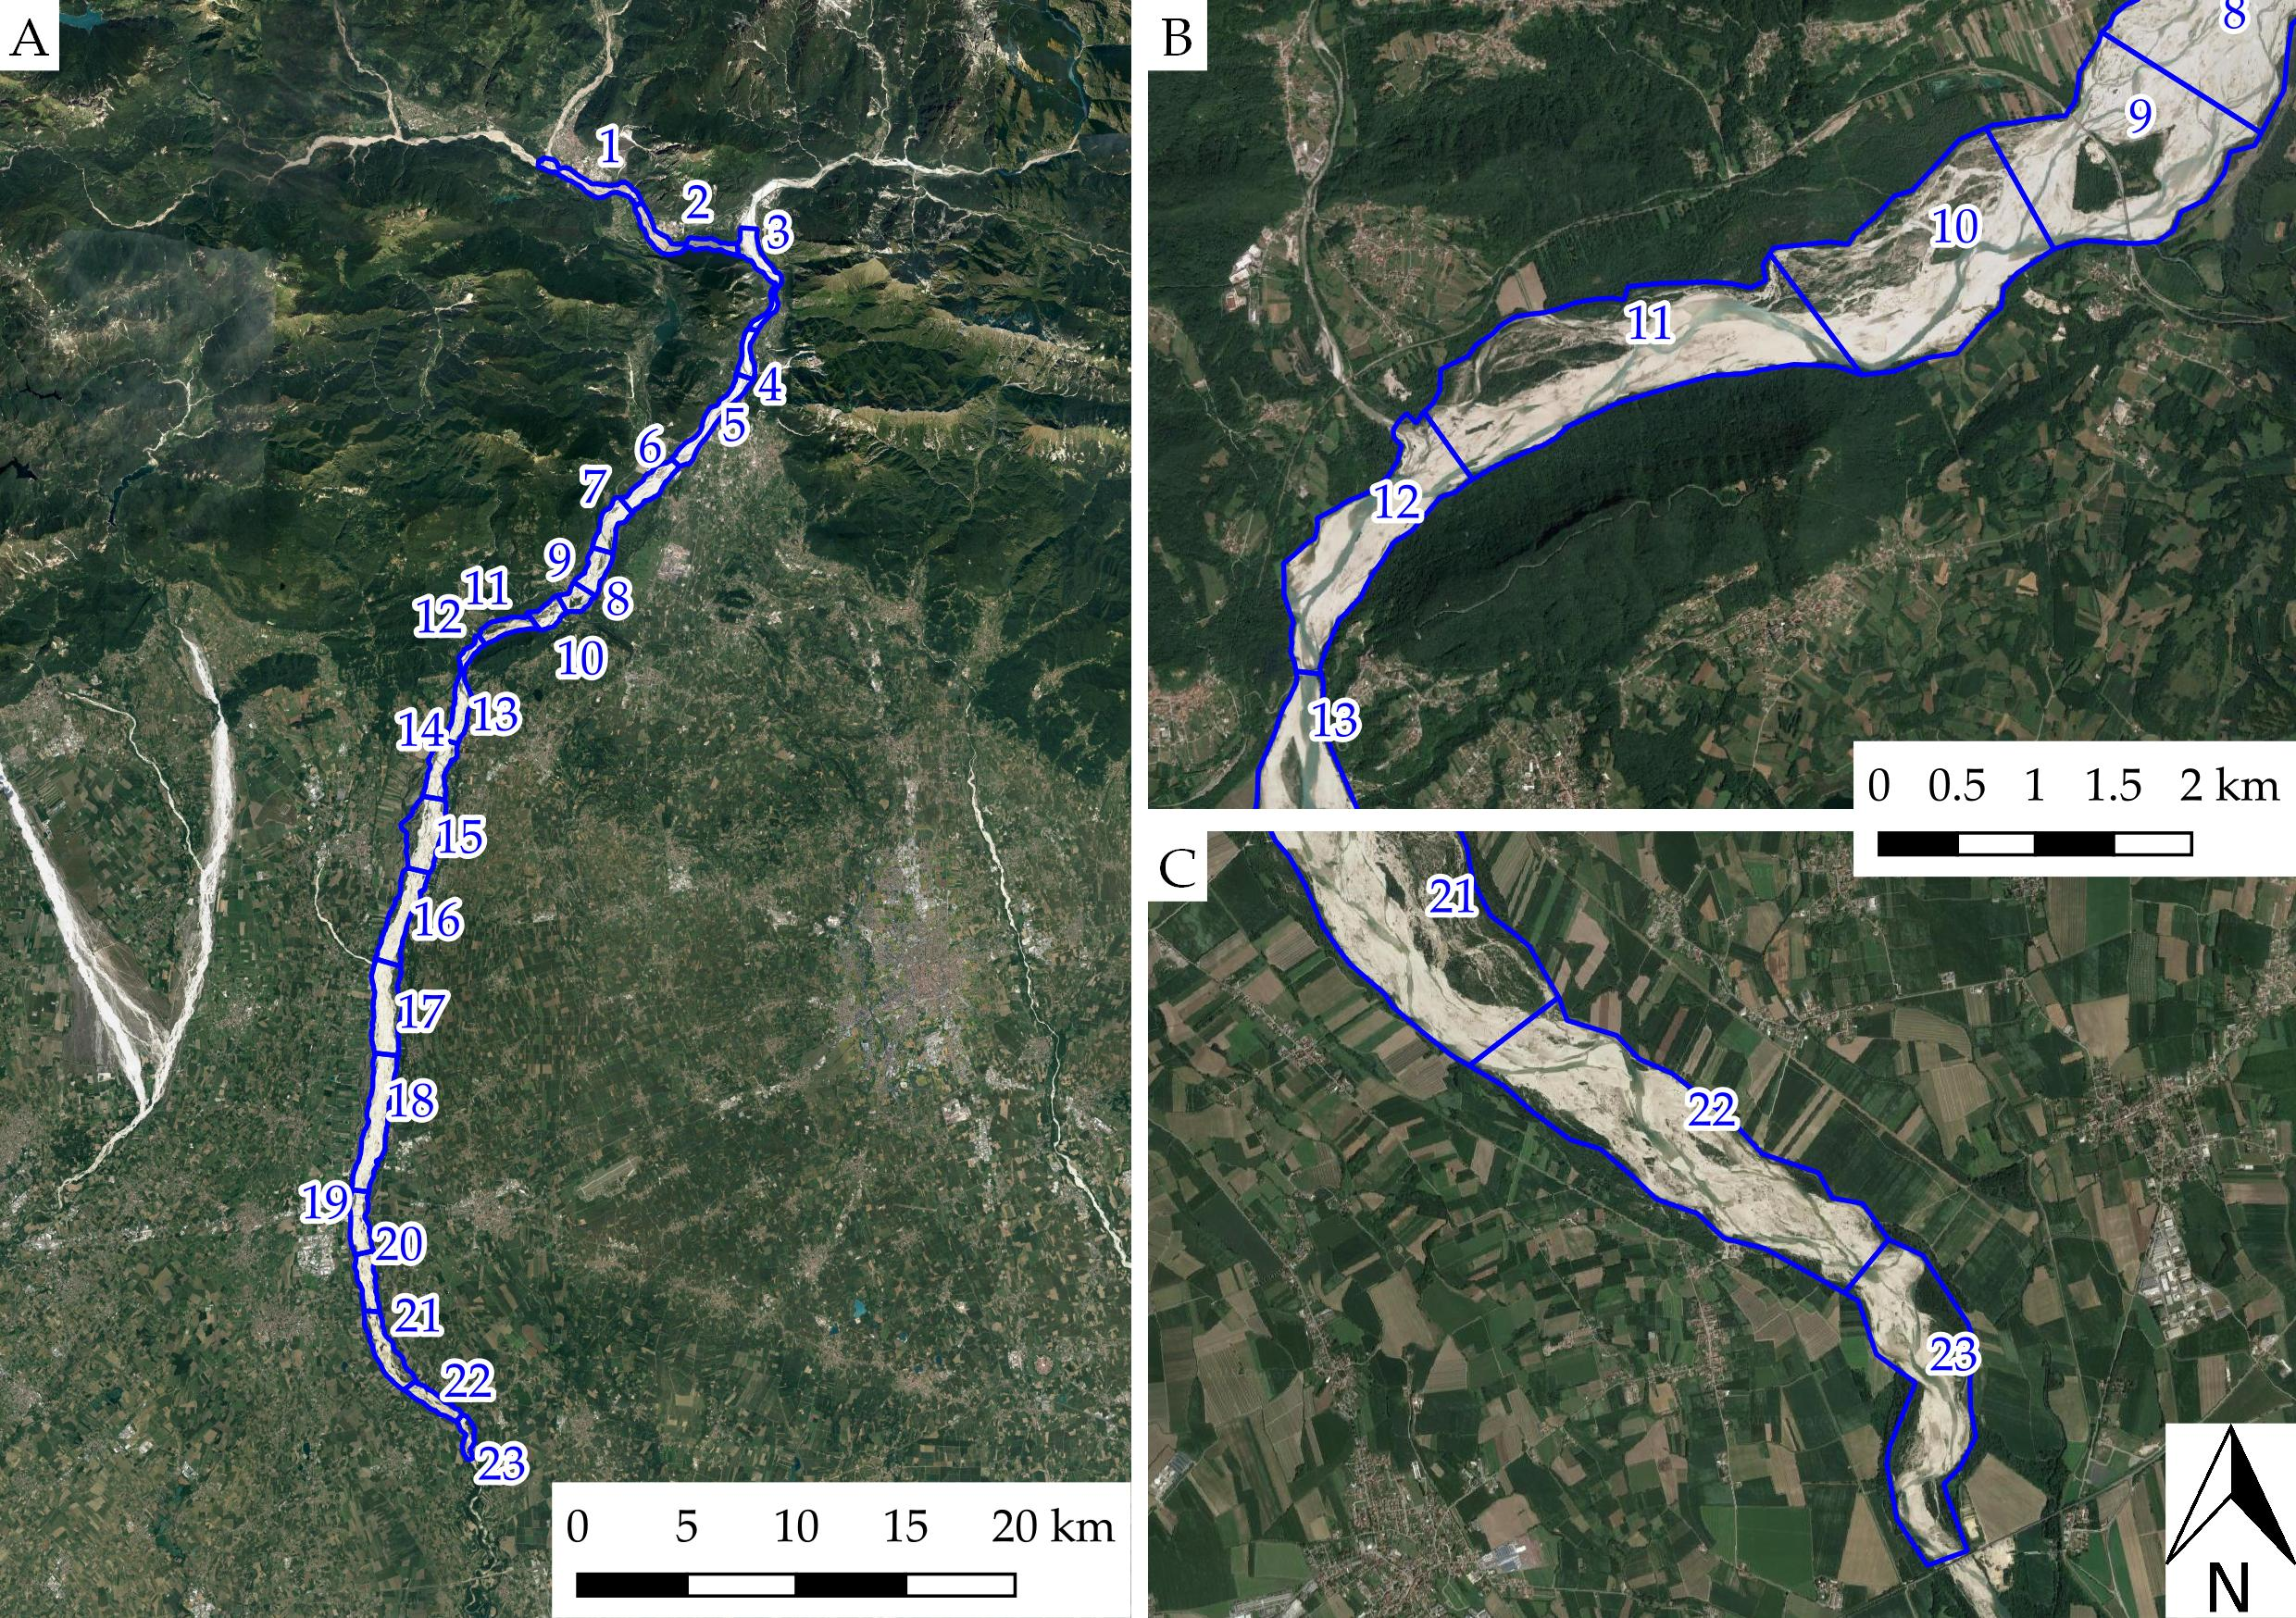
\includegraphics[width=.8\textwidth]{files/tutti_23_tratti.jpeg}
		\caption[immagine con la maschera suddivisa in 23 tratti]{immagine con la maschera suddivisa in 23 tratti; la sezione di monte del tratto~1 corrisponde a Tolmezzo, la sezione di valle del tratto~23 corrisponde al ponte di Madrisio.}
		\label{fig:23-tratti}
	\end{figure}
	%
	%
	\item[isole e \emph{Floodplain}]
	Tramite una procedura semi-automatica e con il supporto di Google Earth, la classe della vegetazione è stata suddivisa in \emph{floodplain} e isole. 
	Tale procedura si basa sul fatto che la maschera computazionale comprende parte della piana alluvionale e che le isole sono completamente circondate dalla ghiaia dell'alveo durante periodi di magra.
	\\
	Successivamente, un controllo visivo del risultato e una correzione manuale di alcune celle hanno permesso sia di distinguere correttamente le isole, sia di evitare che isole molto prossime alla \emph{floodplain} ne fossero considerate parte; la classe delle celle corrette è stata aggiunta alla classificazione.
	%
	%
	\item[Nuvole e nodata] Alcune immagini presentano una lieve copertura nuvolosa che si estende nella maschera; queste zone sono state manualmente delimitate poiché presentano valori NDVI alterati.
	\\
	Altre immagini hanno un'estensione limitata rispetto alla maschera; questo porta ad avere aree prive di dati (\texttt{nodata}).
	\\
	Alla classificazione sono state aggiunte la classe delle nuvole e dei \texttt{nodata}.
	%
	%
	\item[Classificazione finale dei tratti] La \vref{tab:class_tratti} mostra le classi in cui è stato classificato ognuno dei 23~tratti; la \vref{fig:class_is_fl} ne mostra un esempio.
	%
	\begin{table}[ht]
		\centering
		\begin{tabular}{
			c 
			c
			}
			\toprule
			\textbf{Macroclasse}	&	\textbf{Classe}	\\
			\midrule
			Vegetazione		&	Isola	\\
							&	Floodplain	\\
			Alveo attivo	&	Cella corretta	\\
							&	Ghiaia	\\
							&	Canale	\\
			Altro			&	Nuvola	\\
							&	Nodata	\\
			\bottomrule
		\end{tabular}
		\caption[classificazione dell'area dei tratti]{classificazione finale dell'area di ogni tratto all'interno della maschera computazionale.}
		\label{tab:class_tratti}
	\end{table}
	%
	\begin{figure}[ht]
		\centering
		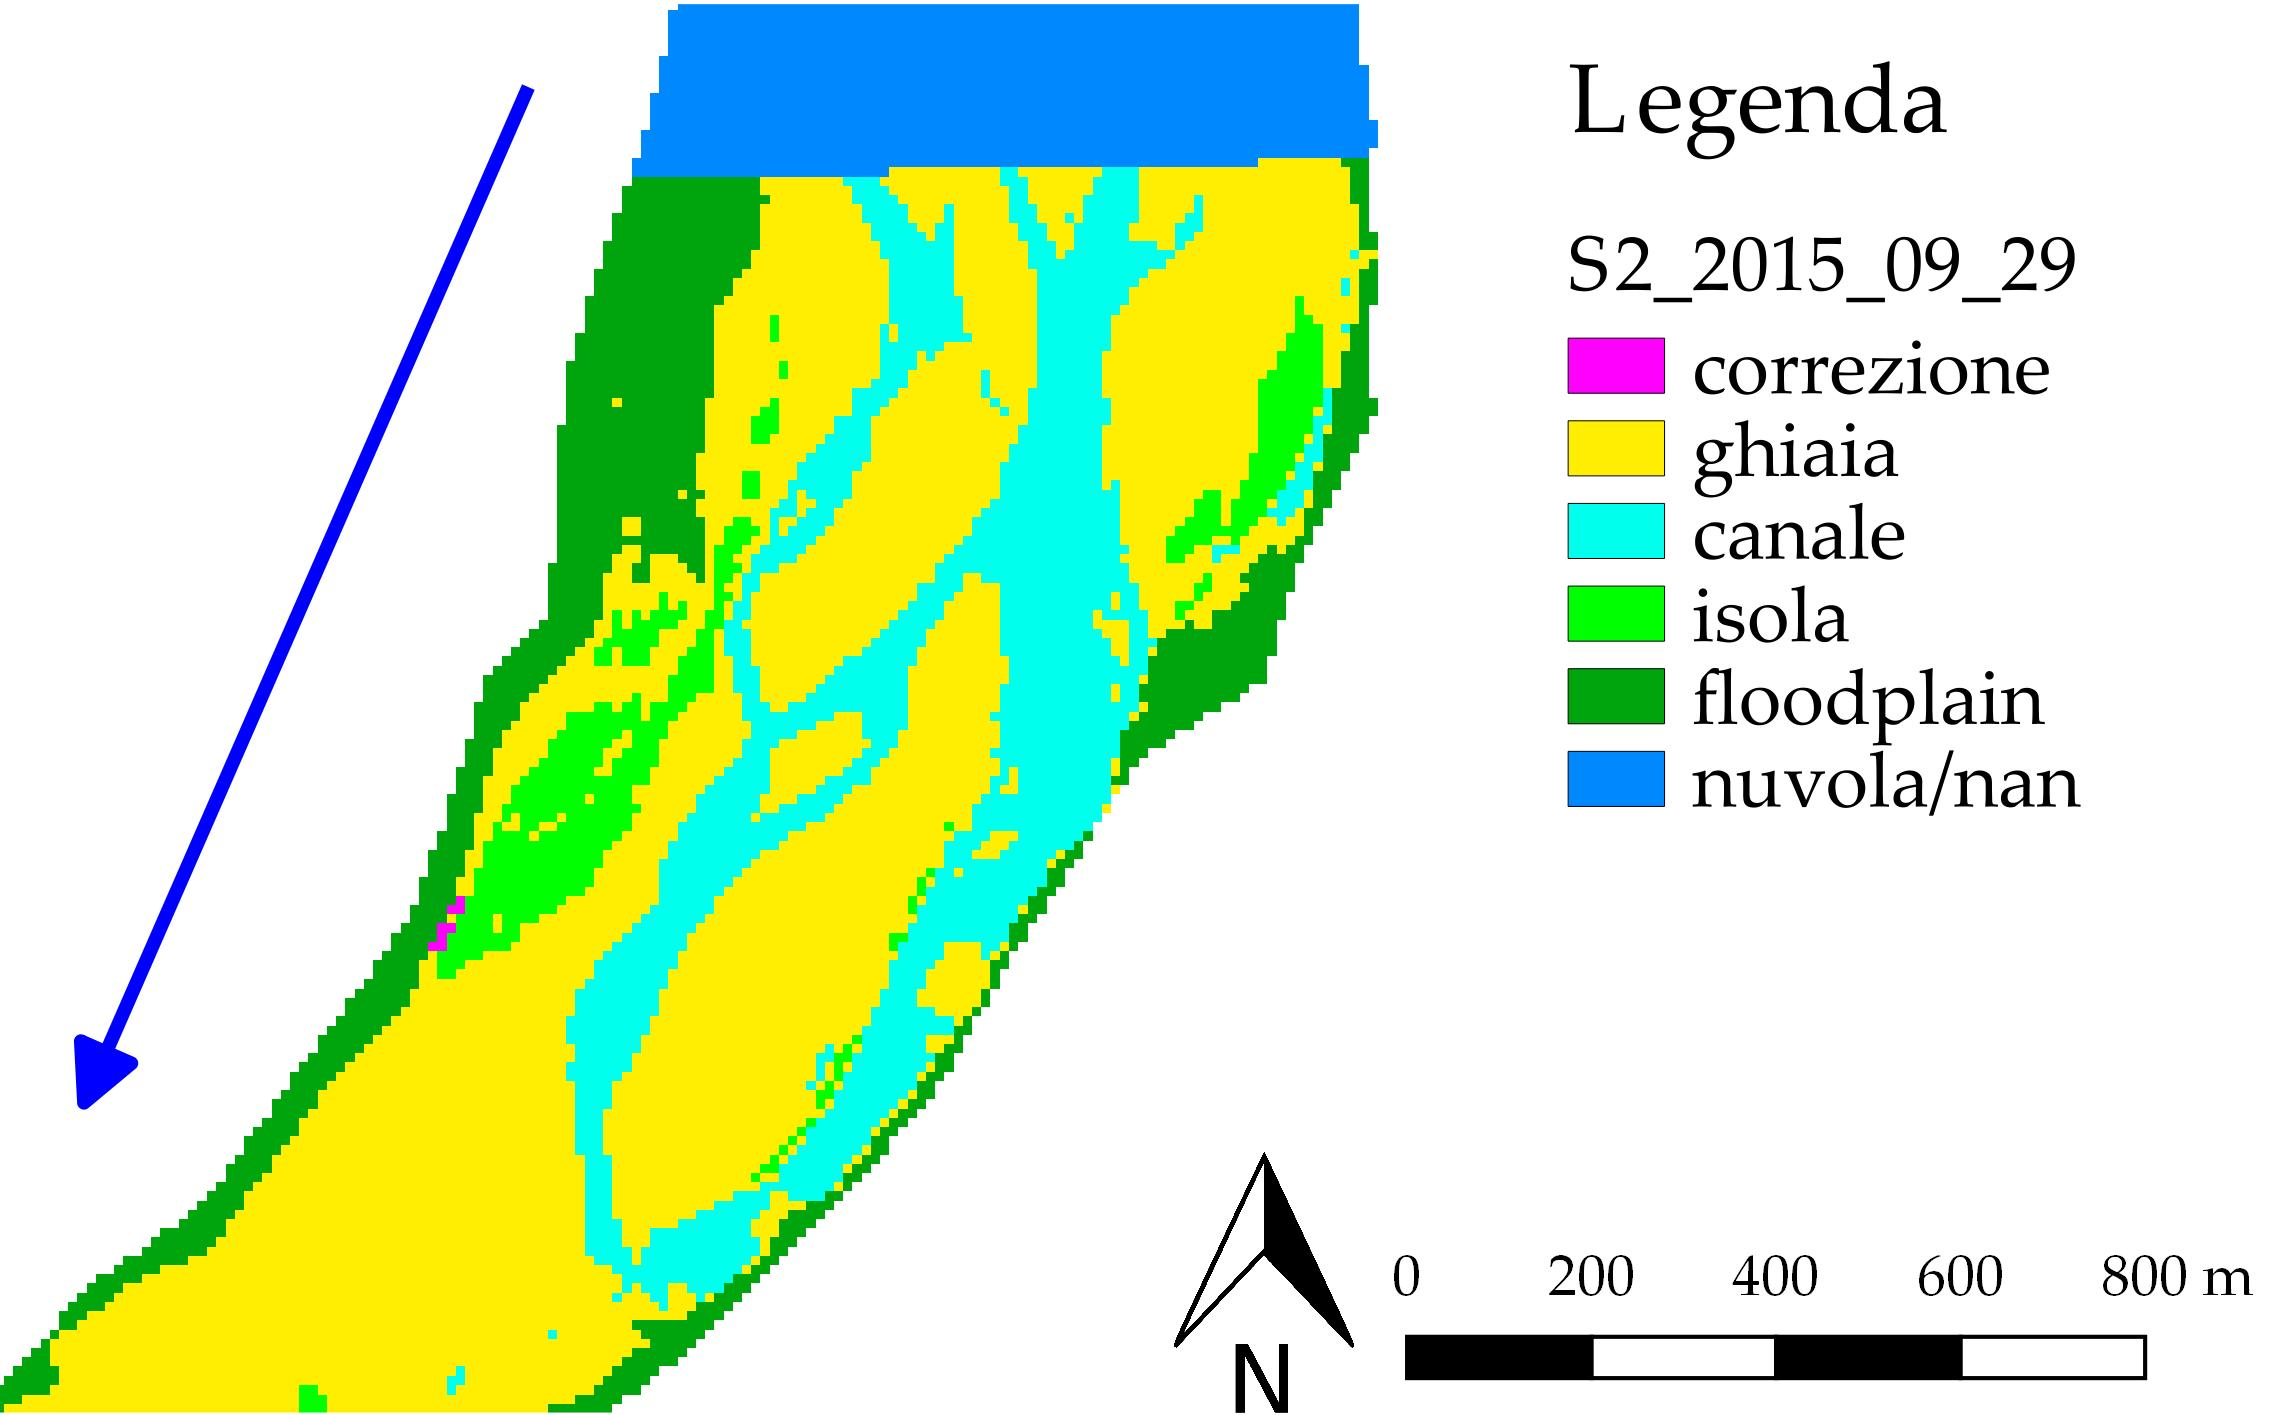
\includegraphics[width=.8\textwidth]{files/esempio_class_is_fl.jpeg}
		\caption[esempio della classificazione dell'area dei tratti]{esempio della classificazione dell'area dei tratti; la zona raffigurata si colloca a ridosso del ponte autostradale a valle di Braulins.}
		\label{fig:class_is_fl}
	\end{figure}
	%

Al fine di validare la precedente procedura di controllo e correzione della distinzione isole - \emph{floodplain}, si è osservato per ogni tratto l'andamento temporale della larghezza media~$B$, esprimibile semplicemente come il rapporto dell'area dell'alveo di ogni tratto (somma dell'alveo attivo e delle isole) per la sua lunghezza seguendo la corrente:
	%
	\begin{equation}
		\label{eq:larghezza-tratto}
		B = \frac{\text{Area alveo}}{Lunghezza} 
		\quad .
	\end{equation}
	% 
	Si è verificato che la larghezza~$B$ rimanesse costante nel tempo, indice di una corretta classificazione tra isole e \emph{floodplain}. 
	La~$B$ non rimane costante solo nel caso di distacco di isole o di fusione di isole nella piana. 
	\\
	La \vref{fig:b-media-7-e-15} mostra l'andamento temporale della~$B$ dei tratti~7 e~15: nel primo tratto, in cui non si osserva alcuna variazione sensibile dell'alveo, la~$B$ oscilla solo di qualche decina di metri; nel secondo si assiste alla progressiva fusione di una grande isola nella \emph{floodplain}, e questo lo si vede proprio nella diminuzione della~$B$. Ciò che conta non è quanto è largo l'alveo, ma quanto cambia la larghezza.
	%
	\begin{figure}
		\centering
		\begin{tikzpicture}
	\begin{axis}[
		width = 0.6\textwidth,
		height = 0.5\textwidth,
		date coordinates in = x,
		xticklabel = {\year},
		xticklabel style = {
			rotate = 80,
			anchor = near xticklabel
		},
		xtick distance = 730,
		enlarge x limits = 0.05,
		enlarge y limits = 0.01,
		%ymax = 3.7,
		%ymin = -0.1,
		%ytick distance = 0.5,
		ylabel = {Larghezza media dell'alveo \si{[\m]}},
		grid = major,
		]
		\addplot+
        	[blue]
        	table [x=data, y=tr_7] {graphics/data/Larghezze_medie_alveo.txt};
        \addlegendentry{Tratto 7}
        
		\addplot+
        	[orange]
        	table [x=data, y=tr_15] {graphics/data/Larghezze_medie_alveo.txt};
        \addlegendentry{Tratto 15}
	\end{axis}
\end{tikzpicture}

		\quad
		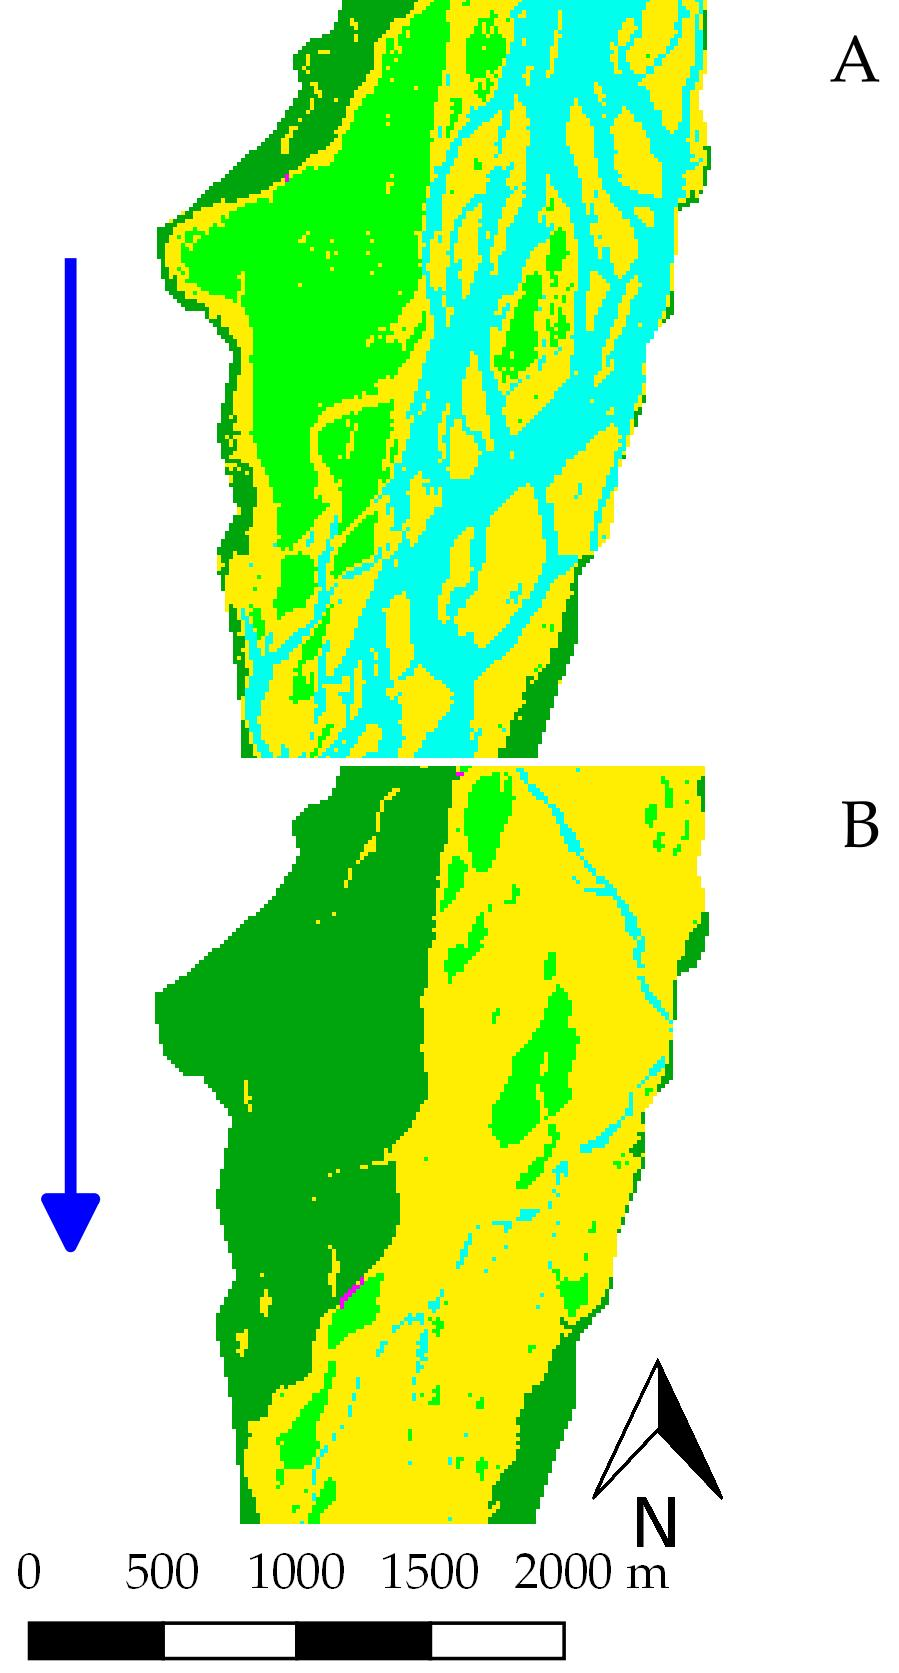
\includegraphics[width=0.3\textwidth]{files/fusione_isola_tr_15.jpeg}
		\caption[andamento temporale di $B$ per i tratti~7 e~15]{a sinistra si vede l'andamento nel tempo della larghezza media dei tratti~7 e~15; la $B$ del tratto~7 oscilla solamente di qualche decina di metri, mentre il tratto~15 riduce improvvisamente la sua $B$ a causa della fusione di una grande isola nella \emph{floodplain}, fenomeno mostrato a destra (A: 2003-11-29, B: 2005-08-30).}
		\label{fig:b-media-7-e-15}
	\end{figure}
	
\end{description}


\begin{comment}
%TODO tenere questa parte? forse la si può togliere
% e mostrare direttamente i risultati sul cambiamento
Con la riclassificazione delle immagini dell'NDVI rispetto alle soglie proposte è stato possibile ottenere la percentuale di alveo coperta da vegetazione per ogni anno. 
Si ricorda, grazie alla maschera applicata, tale copertura include sia isole vegetate sia la parte di piana alluvionale che nel periodo di studio ha esperito fenomeni di erosione della vegetazione e quindi espansione dell'alveo attivo.
Infine, per le immagini l'alveo parzialmente coperto da nuvole, la maschera è stata estesa per escludere tali zone coperte poiché queste presentano valori di NDVI non corretti.
\\
I risultati sono mostrati nel grafico in \vref{graph:class-sat-veg}.


\begin{figure}[ht]
	\centering
	\begin{tikzpicture}
	\begin{axis}[
		width = \textwidth,
		height = 0.5\textwidth,
		date coordinates in = x,
		date ZERO = 2000-01-01,
		xticklabel = {\year},
		xticklabel style = {
			rotate = 80,
			anchor = near xticklabel
		},
		axis y line* = right,
		ymax = 70,
		%ymin = 0,
		ylabel = {Percentuale di vegetazione},
		grid = none,
		]
		\addplot+
        	[red, mark=+, ultra thick]
        	table [x=data, y=veg] {graphics/data/Class_sat_veg-H2O-ghiaia.txt};
	\end{axis}
	
	\begin{axis}[
		width = \textwidth,
		height = 0.5\textwidth,
		date coordinates in = x,
		date ZERO = 2000-01-01,
		xticklabel = {\year},
		xticklabel style = {
			rotate = 80,
			anchor = near xticklabel
		},
		axis y line* = left,
		axis x line = none,
		enlarge x limits = 0.05,
		enlarge y limits = 0.01,
		ymax = 3.7,
		ymin = 2,
		ylabel = {Livello idrometrico},
		grid = none,
		]
		\addplot+
        	[blue, no markers, ultra thin]
        	table [x=data, y=media-gg] {graphics/data/Dati_Villuzza.csv};
	\end{axis}
\end{tikzpicture}

	\caption[andamento dell'areale della vegetazione nelle isole  e nella floodplain]{andamento dell'areale della vegetazione nelle isole e nella floodplain (in rosso). I dati provengono dalla classificazione delle immagini satellitari (\AST{}, \Pl{}, \Se{} e \WV{}). In blu sono mostrati i livelli idrometrici medi giornalieri superiori a~\SI{2}{\m} registrati alla stazione di Villuzza.}
	\label{graph:class-sat-veg}
\end{figure}
% grafico piene 2m+ - %veg tratti (nuovo file comprensivo di tutti i tratti)
\end{comment}



\subsection{Risultati: evoluzione della larghezza}
Utilizzando le mappe di classificazione del terreno all'interno della maschera computazionale, si è ottenuta una larghezza media~$B$ secondo l'equazione~\eqref{eq:larghezza-tratto}.
%TODO \vref{eq:larghezza-tratto}. 
\\
Osservando la variazione temporale di~$B$ è possibile evincere delle traiettorie evolutive sia a livello di singolo tratto, sia a scala più ampia.
Inoltre, considerando la variazione spaziale (da monte verso valle) dell'areale delle isole, sono evidenti i pattern di \emph{upwelling} o \emph{downwelling} utilizzati durante la definizione dei 23~tratti.






\section{Cambiamento delle isole}
A partire dalle mappe di classificazione dell'alveo, sono state ottenute mappe sul cambiamento che le isole hanno, o non hanno, esperito: erosione, crescita, fusione nella \emph{floodplain} o permanenza (nessun cambiamento).
Il risultato sono i dati di partenza per ricercare relazioni con gli eventi di piena.
\\
A tal fine, ogni mappa è stata confrontata con quella temporalmente precedente.
\\
L'analisi si è focalizzata sulle isole, escludendo così la piana alluvionale.

\subsection{Metodi: ottenere il cambiamento}
\paragraph{Limitazioni} \label{par:camb-limiti}
Alcune mappe hanno una estensione limitata oppure presentano zone con copertura nuvolosa: ciò riduce il numero di confronti possibili per alcuni tratti. 
Dalle 23 immagini satellitari (si veda la \vref{tab:date-orto-sat}) si sono ottenute in media 16~immagini per tratto.

Inoltre, le immagini \AST{} non sono correttamente georeferenziate e non sono perfettamente sovrapponibili; l'entità di questo scostamento è dell'ordine di qualche cella.
Questo difetto è di grande importanza poiché per poter investigare l'evoluzione temporale delle isole occorre poter osservare nel tempo ogni cella; se questa si sposta da un'immagine alla successiva, il confronto non è più valido.
\\
La soluzione adottata è stata quella di traslare ogni mappa a nord, sud, est o ovest del numero di celle necessario per poterla sovrapporre alla mappa temporalmente precedente.
L'operazione è stata ripetuta per ogni confronto, per ogni tratto, ed è stata verificata visivamente.
Il massimo errore residuo è di 1~cella di scostamento in pochissime zone nei primi tratti (\numrange[range-phrase={ - }]{1}{4}); data la locale topografia montuosa si è preferito ridurre l'errore a tale entità e tenerlo sotto controllo piuttosto di distorcere la mappa con altre misure di georettifica.
\\
Le altre immagini sono invece correttamente georeferenziate.

Infine, per poter confrontare immagini a diversa dimensione di cella, come le \AST{} a~\SI{15}{\m} con le \Pl{} a~\SI{0.5}{\m}, è stato necessario ricampionare le immagini con la dimensione minore (ad esempio le \Pl{}) alla risoluzione di quelle a dimensione maggiore (le \AST{} o le \Se{}).
\\
Nel ricampionamento l'areale delle isole subisce un incremento o una riduzione, così come l'areale della ghiaia e delle altre classi in quanto nelle celle a dimensione maggiore sono presenti numerose celle a dimensione minore, ognuna con un valore diverso (\vref{fig:ricamp-explanation}).
%
\begin{figure}
	\centering
	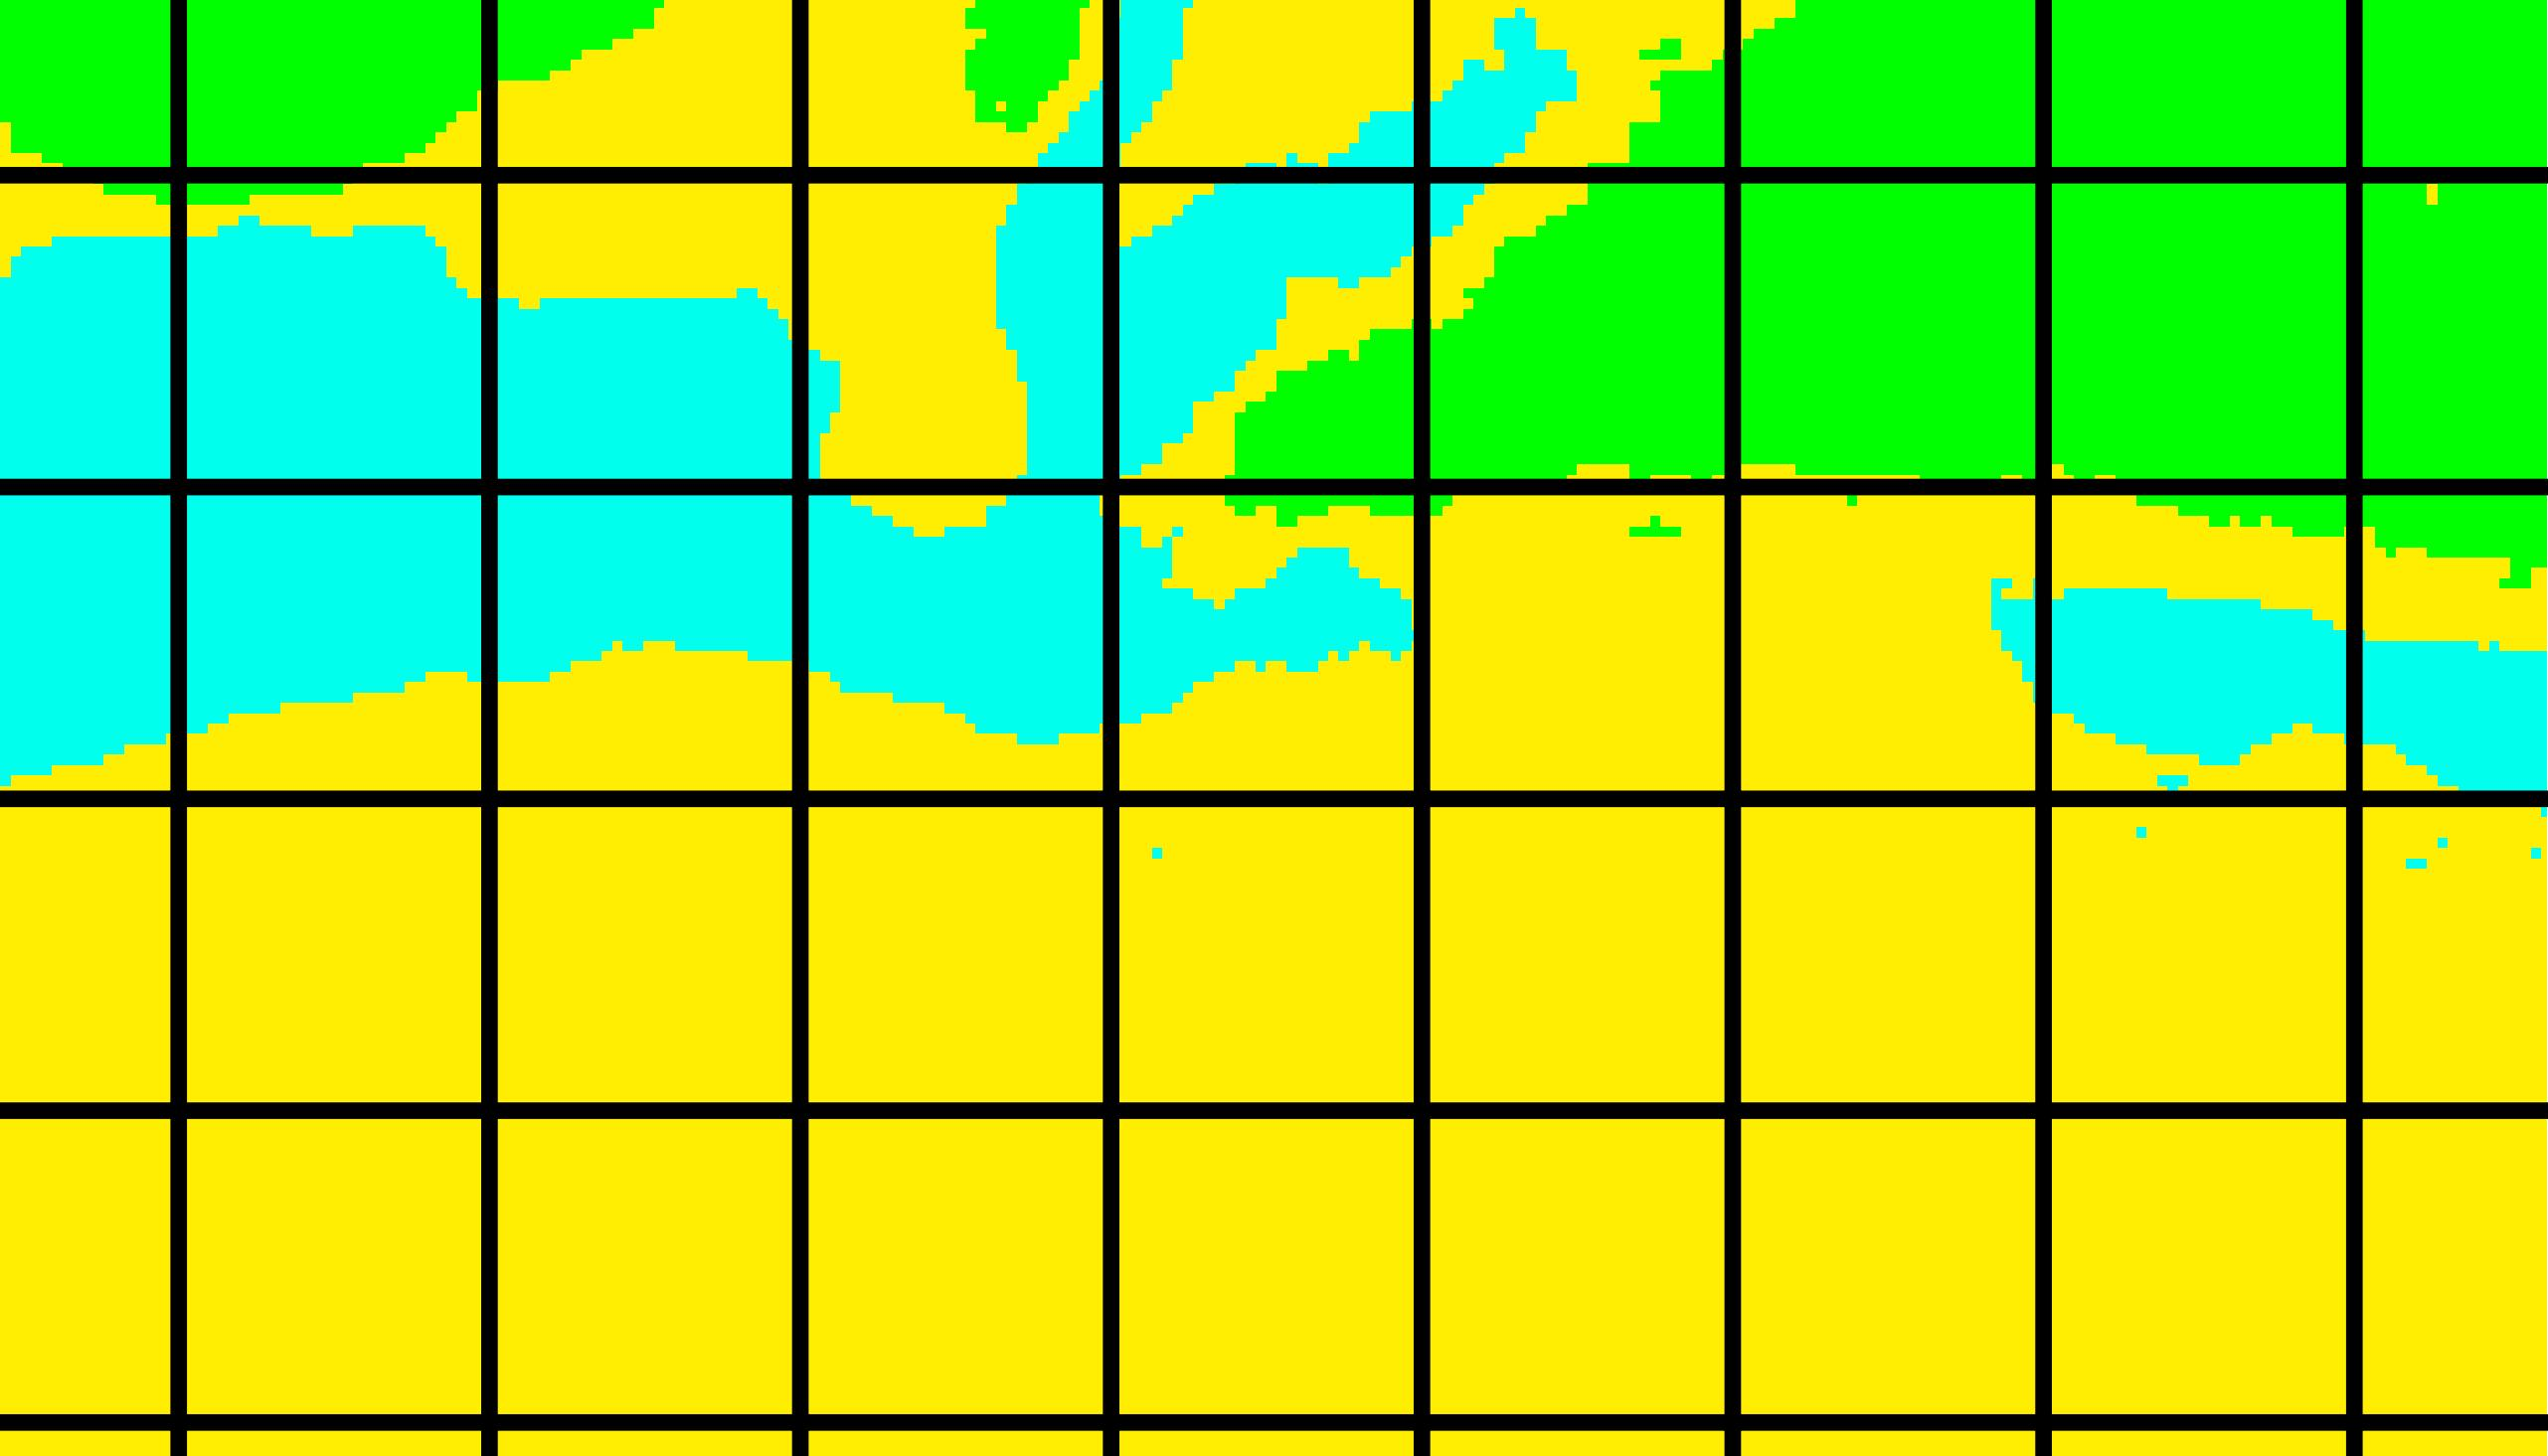
\includegraphics[width=.9\textwidth]{files/ricamp_griglia.jpeg}
	\caption[celle a risoluzione diversa]{immagine \Pl{} 2015-08-13 a~\SI{0.5}{\m} sullo sfondo con la griglia a~\SI{15}{\m} in primo piano; si vede come diverse celle più piccole siano contenute in una singola cella maggiore.}
	\label{fig:ricamp-explanation}
\end{figure}
%
Nel ricampionamento si sceglie quale valore assegnare alla nuova cella più grande in base ai valori delle celle minori; nel presente lavoro si è scelto di assegnare un percentile.
La scelta del percentile è stata effettuata confrontando la radice quadrata della somma dei quadrati residui (RSQR):
%
\begin{equation}
	\label{eq:rad-som-quad-res}
	RSQR = \left\lbrace \sum_{n=1}^{cl} \left[\left( \frac{area_{\mathrm{orig,n}}}{area_{\mathrm{orig,tot}}} - \frac{area_{\mathrm{perc,n}}}{area_{\mathrm{perc,tot}}} \right)^2 \right] \right\rbrace ^ \frac{1}{2}	
\end{equation}
%
dove 
\begin{itemize}
	\item $cl$ è il numero di classi (\vref{tab:class_tratti});
	\item $n$ indica la $n$-esima classe;
	\item $area_{\mathrm{orig,n}}$ e $area_{\mathrm{perc,n}}$ sono rispettivamente l'area della $n$-esima classe nella mappa originale e in quella ricampionata ad un percentile;
	\item $area_{\mathrm{orig,tot}}$ e $area_{\mathrm{perc,tot}}$ sono rispettivamente l'area totale della mappa originale e in quella ricampionata ad un percentile. 
\end{itemize} 
%
Si è scelto di normalizzare l'area di ogni classe per l'area totale per lavorare con percentuali.
\\
Nei ricampionamenti da \SI{0.5}{\m} il $50_\mathrm{mo}$ percentile (mediana) è quello che mostra il minor RSQR ($<\SI{3}{\percent}$); in quelli da \SI{10}{\m} il $75_\mathrm{mo}$ percentile (terzo quartile) è il migliore ($RSQR<\SI{6}{\percent}$). Un esempio del risultato ottenuto è mostrato in \vref{fig:ricampionamento}.
%
\begin{figure}
	\centering
	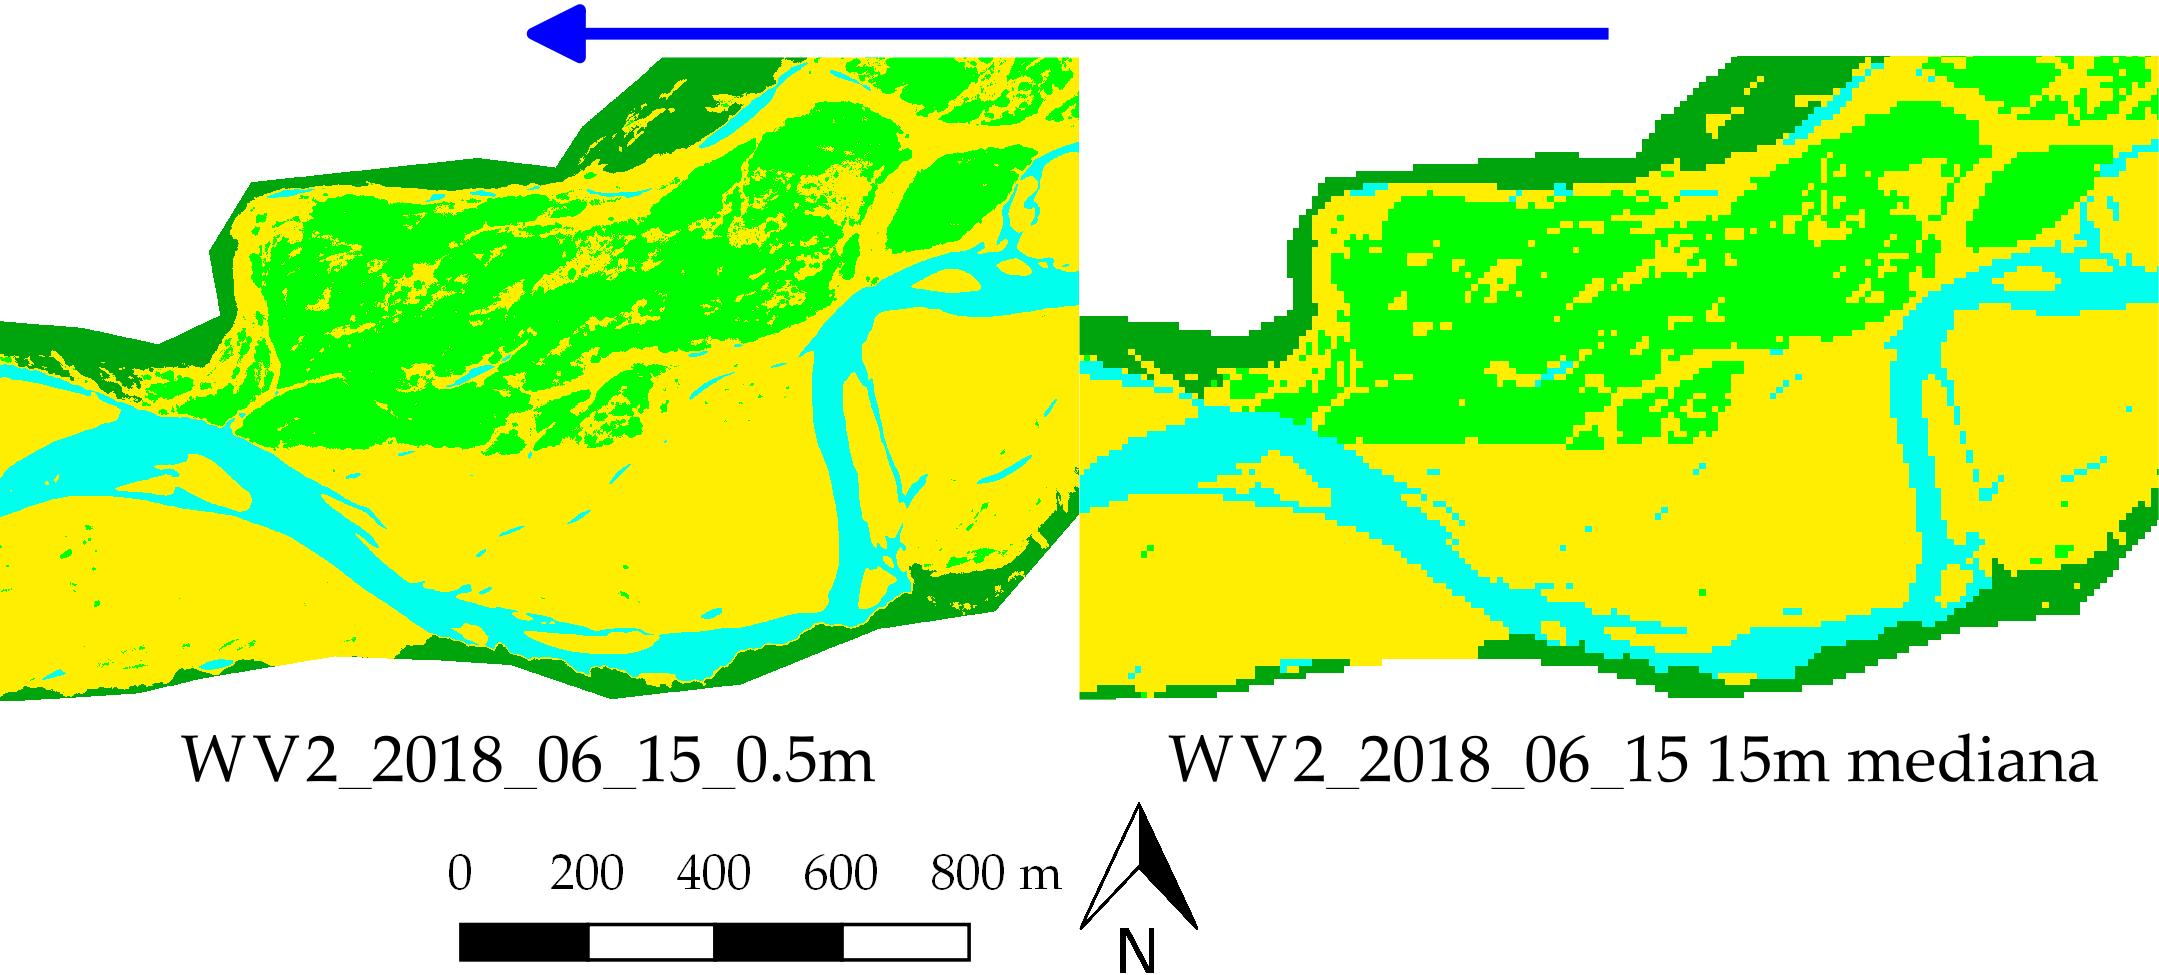
\includegraphics[width=\textwidth]{files/ricamp_class_is_fl.jpeg}
	\caption[confronto originale - ricampionamento]{a sinistra l'immagine \WV{} originale, poco a valle dell'isola di Cornino; a destra la stessa immagine ricampionata distribuendo i valori con la mediana.}
	\label{fig:ricampionamento}
\end{figure} 
%


\paragraph{Confronti validi}
Dalle 23 immagini satellitari è stato possibile ottenere il numero di confronti mostrati in \vref{tab:confronti}. 
I confronti effettuati hanno la massima risoluzione temporale possibile, cioè per ogni tratto si sono confrontate le immagini valide temporalmente più vicine in modo da poter osservare gli effetti cumulati del minor numero possibile di eventi di piena.
%
\begin{table}
	\centering
	\begin{tabular}{
		S[table-format=2.0] 
		S[table-format=2.0]
		c 
		c}
		\toprule
		\textbf{Tratto}	&	\textbf{Confronti}	&	\textbf{Primo}		&	\textbf{Ultimo}	\\
						&	\textbf{validi}		&	\textbf{confronto}	&	\textbf{confronto}	\\
		\midrule
		1	&	13	&	2000-09-17/2003-06-22	&	2016-09-13/2017-04-21	\\
		2	&	13	&	2000-09-17/2001-06-17	&	2016-09-13/2017-04-21	\\
		3	&	16	&	2000-09-17/2001-06-17	&	2016-09-13/2017-04-21	\\
		4	&	16	&	2000-09-17/2001-06-17	&	2016-09-13/2017-04-21	\\
		5	&	16	&	2000-09-17/2001-06-20	&	2016-09-13/2017-04-21	\\
		6	&	18	&	2000-09-17/2001-06-17	&	2017-04-21/2018-06-15	\\
		7	&	18	&	2000-09-17/2001-06-17	&	2017-04-21/2018-06-15	\\
		8	&	19	&	2000-09-17/2001-06-17	&	2017-04-21/2018-06-15	\\
		9	&	18	&	2000-09-17/2002-05-18	&	2017-04-21/2018-06-15	\\
		10	&	18	&	2000-09-17/2002-05-18	&	2017-04-21/2018-06-15	\\
		11	&	18	&	2000-09-17/2002-05-18	&	2017-04-21/2018-06-15	\\
		12	&	18	&	2000-09-17/2002-05-18	&	2017-04-21/2018-06-15	\\
		13	&	18	&	2000-09-17/2002-05-18	&	2017-04-21/2018-06-15	\\
		14	&	21	&	2000-09-17/2002-05-18	&	2017-04-21/2018-06-15	\\
		15	&	16	&	2000-09-17/2002-06-12	&	2016-09-13/2017-04-21	\\
		16	&	16	&	2000-09-17/2002-06-12	&	2016-09-13/2017-04-21	\\
		17	&	16	&	2000-09-17/2002-06-12	&	2016-09-13/2017-04-21	\\
		18	&	16	&	2000-09-17/2002-06-12	&	2016-09-13/2017-04-21	\\
		19	&	13	&	2000-09-17/2002-06-12	&	2016-09-13/2017-04-39	\\
		20	&	13	&	2000-09-17/2002-06-12	&	2014-09-28/2015-09-11	\\
		21	&	13	&	2000-09-17/2002-06-12	&	2014-09-28/2015-09-11	\\
		22	&	13	&	2000-09-17/2002-06-12	&	2014-09-28/2015-09-11	\\
		23	&	12	&	2002-06-12/2003-06-22	&	2014-09-28/2015-09-11	\\
		\bottomrule
	\end{tabular}
	\caption[confronti effettuati]{confronti effettuati con le 23 immagini satellitari a disposizione per ottenere dati sul cambiamento delle isole.}
	\label{tab:confronti}
\end{table}
%

\paragraph{Classi del cambiamento}
In ogni confronto ci si è concentrati sul ciò che è successo alle isole, definendo quindi le seguenti 4~classi (si veda anche la \vref{tab:class_tratti}):
%
\begin{itemize}
	\item erosione (da isola ad alveo attivo);
	\item crescita (da alveo attivo ad isola);
	\item fusione nella \emph{floodplain} (da isola a \emph{floodplain});
	\item distaccamento dalla \emph{floodplain} (da \emph{floodplain} a isola);
	\item nessun cambiamento (da isola a isola).
\end{itemize}
%
Un esempio di questa classificazione è riportato nella \vref{fig:confr-class-is-fl}.
%
\begin{figure}
	\centering
	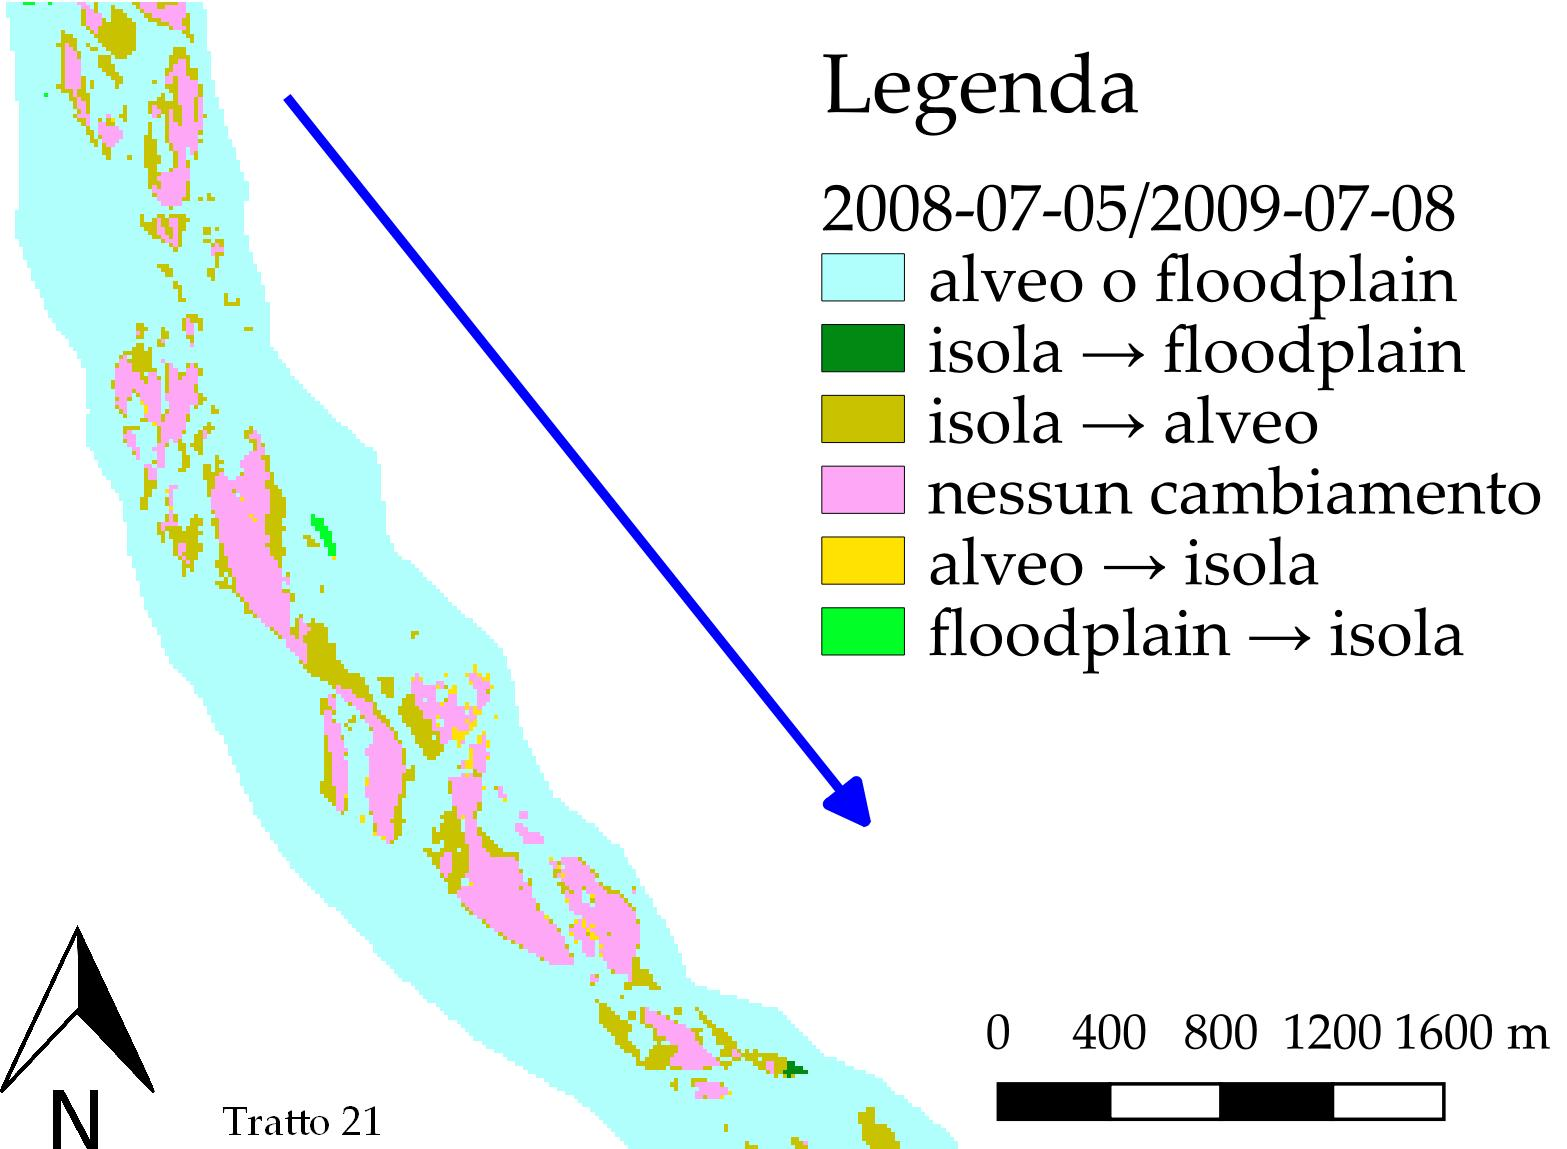
\includegraphics[width=.8\textwidth]{files/confr_class_is_fl.jpeg}
	\caption[esempio di mappa di cambiamento]{esempio di mappa di cambiamento ottenuta con il confronto tra le immagini \AST{} 2008-07-05 e 2010-09-29. Si possono osservare tutti i cambiamenti possibili; la prima classe serve solamente a visualizzare l'area della maschera computazionale. Il tratto mostrato è posto qualche \si{\kilo\m} a monte del ponte di Madrisio.}
	\label{fig:confr-class-is-fl}
\end{figure}
%


\subsection{Risultati: eventi eccezionali}
Dall'osservazione dell'idrogramma in \vref{graph:livelli-orto-sat} (riportato \vpageref{graph:tr-17-camb}) si può ipotizzare che le piene maggiori, come quelle avvenute verso la fine degli anni~2012 e~2014, siano quelle che abbiano asportato il maggior quantitativo di isole.
\\
I grafici in \vref{graph:tr-17-camb} mostrano alcuni risultati ottenuti dalle mappe di cambiamento per il tratto~17, posto nel tratto vallivo immediatamente a valle della confluenza con il torrente Cosa.
I dati sono rappresentati con due simboli: il pallino rappresenta la data finale di ogni confronto, mentre la croce indica la data iniziale; 
chiaramente il pallino di un confronto ha la stessa data della croce del confronto successivo. 
La croce serve solamente a sapere quanto dura ogni confronto; il pallino è il dato vero e proprio.
I dati sono normalizzati per l'areale delle isole nell'immagine \AST{} del 2000-09-17.
\\
Ciò che si vede è una spiccata crescita a cavallo degli anni~2006 e~2008, seguita da una erosione delle medesime proporzioni.
Dall'altra parte, nonostante la maggior intensità e durata le piene del 2012 e del~2014 hanno eroso meno di quanto ci si aspettava.
%
\begin{figure}
	\centering
	\begin{tikzpicture}
	%\begin{groupplot}
	\begin{axis}[
		%name = orto-sat,
		axis y line* = right,
		axis x line* = top,
		%height = .3\textwidth,
		width = \textwidth,
		date coordinates in = x,
		%symbolic y coords = {ASTER,PLEIADES,SENTINEL2,G-EARTH},
		xticklabel = {\year-\month-\day},
		xtick = data,
		ytick = data,
		xticklabel style = {
			rotate = 90,
			anchor = near xticklabel
		},
		enlarge x limits = 0.05,
		enlarge y limits = 0.01,
		ylabel = {Fonte},
		ymax = 3.6,
		ymin = -0.1,
		grid = none,
		only marks,
		]
		\addplot table [x=data, y=numero] {graphics/data/data-orto-sat.txt};
	\end{axis}
	%
	\begin{axis}[
		%name = stages,
		%at = {($(orto-sat.south)-(0,2cm)$)},
		%anchor = north,
		axis y line* = left,
		width = \textwidth,
		date coordinates in = x,
		xticklabel = {\year-\month-\day},
		xticklabel style = {
			rotate = 45,
			anchor = near xticklabel
		},
		enlarge x limits = 0.05,
		enlarge y limits = 0.01,
		ymax = 3.6,
		ymin = -0.1,
		ylabel = {Livello idrometrico},
		grid = major,
		no markers,
		]
		\addplot table [x=data, y=media-gg] {graphics/data/Dati_Villuzza.csv};
	\end{axis}
\end{tikzpicture}
	\\
	\begin{tikzpicture}
	\begin{groupplot}[
		group style = {
			group size = 2 by 1,
			ylabels at = edge left,
			x descriptions at = edge bottom,
			horizontal sep = 1.1cm,
			vertical sep = 0.1cm,
		},
		width = 0.5\textwidth,
		height = 0.5\textwidth,
		date coordinates in = x,
		xticklabel = {$\year$},
		xticklabel style = {
			rotate = 80,
			anchor = near xticklabel
		},
		xtick distance = 731,
		ymax = 0.75,
		ylabel = {Cambiamento/Isole iniziali \si{[\percent]}},%\si{[\m\tothe{2}]}},
		grid = major,
		]
	\nextgroupplot % tr_17_accrescimento
		\addplot+
        	[only marks, blue]
        	table [
        		x=data_fine, 
        		y expr=\thisrow{alv->is}/808650.0
        		] {graphics/data/tr_17_camb_eros_accr.txt};
		\addplot+
        	[only marks, mark=x, black]
        	table [
        		x=data_ini, 
        		y expr=\thisrow{alv->is}/808650.0
        		] {graphics/data/tr_17_camb_eros_accr.txt};
        \node [fill = white, draw = black, anchor = south west] 
        	at (axis description cs: 0.05,0.8) {Accr.};
	\nextgroupplot % tr_17_erosione
		\addplot+
        	[only marks, blue]
        	table [
        		x=data_fine, 
        		y expr=\thisrow{is->alv}/808650.0,
        		] {graphics/data/tr_17_camb_eros_accr.txt};
		\addplot+
        	[only marks, mark=x, black]
        	table [
        		x=data_ini, 
        		y expr=\thisrow{is->alv}/808650.0,
        		] {graphics/data/tr_17_camb_eros_accr.txt};
        \node [fill = white, draw = black, anchor = south west] 
        	at (axis description cs: 0.05,0.8) {Eros.};
	\end{groupplot}
\end{tikzpicture}

	\caption[cambiamenti esperiti dalle isole nel tratto~17]{cambiamenti esperiti dalle isole nel tratto~17 rappresentati come percentuale rispetto all'areale delle isole nella prima immagine utile. 
	Si nota il dato relativo al confronto 2008-07-05/2010-09-29, particolarmente elevato e di pari entità tra crescita ed erosione.}
	\label{graph:tr-17-camb}
\end{figure}
%
Questa osservazione può trovare la seguente giustificazione: il periodo privo di piene con livello al disopra dei \SI{2}{\m} tra fine del 2004 e la fine del 2008 è stato favorevole per l'insediamento di nuova vegetazione;
le macchie vegetate sono diventate visibili da satellite solamente quando le piante hanno sviluppato una chioma sufficientemente ampia, cioè dopo qualche anno, nell'immagine del 2008-07-05;
questa più recente vegetazione si è espansa sulle barre e sulle forme morfologiche a quota minore rispetto alle isole più vecchie;
con questi fatti, la prima piena che è giunta ha facilmente portato via tutte queste isole giovani e basse.
\\
Occorre quindi ragionare non solo in termini di singoli eventi di piena, ma estendere le proprie considerazioni all'intero idrogramma, al periodo di tempo tra piene oltre un certo livello, alla loro frequenza, poiché sono questi i fattori che possono determinare le dinamiche delle isole.
Il periodo 2005-2008 privo di grandi piene può essere considerato un evento tanto importante quanto la piena lunga ed intensa del mese di Novembre, 2014.

%TODO c'è un trend: i tratti con upwelling sono quelli che si vegetano di più


Da queste osservazioni il passo successivo è naturale: trovare la composizione delle isole in termini di età e riflettere se è la vegetazione più giovane quella ad essere più facilmente erosa.




\section{Età della vegetazione nelle isole}
Utilizzando le mappe del cambiamento esperito dalle isole si possono ottenere mappe che indicano un'età approssimativa della vegetazione che compone queste isole. 
\\
L'ipotesi che si vuole verificare è che sia la vegetazione più giovane quella ad essere maggiormente erosa in quanto può essere divelta più facilmente.
Non si esclude tuttavia di osservare erosione anche di vegetazione matura poiché le isole poste in corrispondenza dell'estradosso di un canale curvo sono soggette a scavo laterale.

\subsection{Metodi: estendere i confronti e ottenere un'età}
\paragraph{Limiti}
Con le immagini satellitari utilizzate non è possibile distinguere i singoli alberi che compongono le isole; se con le immagini a miglior risoluzione si distinguono gli arbusti isolati, non si può certo ottenere una stima dell'età tanto precisa quanto quella fornita da un carotaggio del tronco.
In più, una cella è classificata come vegetazione solo quando le piante al suo interno presentano una chioma sufficientemente grande da occupare gran parte della cella; pertanto le immagini con celle di \SI{10}{\m} o addirittura \SI{15}{\m} non possono mostrare che grandi macchie di vegetazione.
Prima dei \SI{3}{\anni} una pianta di salice generalmente non ha fronde molto estese.
\\
Occorre poi tenere in conto che le piante crescono differentemente in base alle condizioni ambientali: periodi di stress idrico o termico rallentano la crescita, così come il parziale seppellimento con ghiaia dovuto ad eventi di piena; una falda non troppo profonda la cui altezza varia lentamente, terreno di granulometria sottile con sabbia e buone temperature sono invece fattori favorevoli alla crescita \squarecite{Gurnell:2001-island-formation}.

Si crede che ciò che possa accadere è che fino ad una certa età, circa \SI{3}{\anni}, la nuova vegetazione non sia visibile dal satellite. 

Le mappe del cambiamento sono state ottenute dalle mappe di classificazione; non essendo le seconde correttamente georeferenziate, neanche le prime lo sono. L'errore residuo nel processo di correzione è di 1~cella.

Infine, per poter confrontare nel corso degli anni ogni cella, le mappe del cambiamento sono state ricampionate alla risoluzione più bassa, corrispondente a celle di~\SI{15}{\m} di lato. Si è proceduto come mostrato nel paragrafo \ref{par:camb-limiti} ottenendo valori $RSQR < \SI{1.5}{\percent}$.
 

%TODO le piante crescono diversamente in base alle condizioni ambientali (cita articolo Gurnell?) → definire un'età in base al tempo di osservazione è un approccio limitato (qualche altro lavoro simile)

\paragraph{Obiettivo ed approccio} 
Date le precedenti premesse, bisogna riflettere su ciò che si vuole ottenere: dividere la vegetazione in classi di età.
Si vuole sapere quanta vegetazione giovane è stata erosa; non importa se questa ha esattamente \SI{3}{\anni} o \SI{4}{\anni}, l'importante è che sia grossomodo classificata come giovane.

Ogni mappa del cambiamento è formata dalle informazioni contenute in due mappe: quella più vecchia e quella più recente. La distanza temporale tra queste due mappe definisce il periodo di osservazione.
\\
Per la mappa del cambiamento più vecchia, l'età della vegetazione delle isole è stata arbitrariamente essere pari al periodo di osservazione, cui si sono aggiunti \SI{3}{\anni}.
\\
Per le mappe via via più recenti, l'età nelle celle delle isole che non sono cambiate è pari al periodo di osservazione sommato all'età precedente; per le celle si sono vegetate a partire dall'alveo l'età è pari al periodo di osservazione con l'aggiunta di \SI{3}{\anni}, ritenuto il periodo minimo affinché un insieme di piante diventi visibile per il satellite.

\medskip
L'approccio di definire un'età in base al periodo di osservazione è limitato, in particolare per le mappe più vecchie poiché non è possibile tener conto della vegetazione che era presente antecedentemente alla prima immagine valida;
si ritiene che a partire dalla $4^a$ o $5^a$ mappa di età il metodo inizi ad essere affidabile (generalmente quindi dalla mappa di età del 2007-09-21).
Per gli scopi della ricerca questo approccio risulta essere sufficiente.

\paragraph{Validazione}
Il CSM (\emph{Canopy Surface Model}) è il modello digitale della copertura arborea; similmente al DEM, mostra delle quote; queste sono tuttavia riferite all'altezza della vegetazione sopra il terreno.
\\
È generalmente sensato affermare che piante più mature abbiano un'altezza maggiore di piante giovani.
Quindi si sono utilizzate le informazioni del CSM relativo alla ortofoto del 2013-10-22 per verificare che nelle celle della mappa di età della vegetazione del 2013-09-05 l'altezza fosse all'incirca proporzionale all'età.
%TODO grafico con i quantili

\subsection{Risultati: un trend per la vegetazione erosa}
I grafici in \vref{graph:distr-eta} mostrano la distribuzione di età della vegetazione nelle isole in termini di areale occupato; per gli scopi del lavoro ci si limita a definire 3~classi di vegetazione:
%
\begin{itemize}
	\item giovane, con meno di \SI{5}{\anni};
	\item intermedia, con età compresa tra \SIrange[range-phrase={ e }]{5}{10}{\anni};
	\item matura, con più di \SI{10}{\anni}.
\end{itemize}

%TODO da migliorare (togliere la descrizione all'asse y?)
%
\begin{figure}
	\centering
	\begin{tikzpicture}
	\begin{groupplot}[
		group style = {
			group size = 1 by 3,
			ylabels at = edge left,
			x descriptions at = edge bottom,
			xticklabels at = all,
			horizontal sep = 1.1cm,
			vertical sep = 1cm,
		},
		width = \textwidth,
		%height = 0.6\textwidth,
		xbar stacked,
		%bar width = 5pt,
		%enlarge x limits = 0.05,
		%enlarge y limits = 0.01,
		xmin = 0,
		scaled x ticks = false,
		xtick distance = 1e5,
		xlabel = {Area occupata \si{[\m\tothe{2}]}},
		ylabel = {Mappa di età},
		grid = major,
		]
		\nextgroupplot [% tratto_8
			height = 0.45\textwidth,
			legend style = {
				at = {(0.5,1.05)},
				legend columns = 3,
				anchor = south
			}, 
			legend entries = {giovane, intermedia, matura},
			symbolic y coords = {
				2008-07-05, 2009-07-08, 
				2012-08-01, 2013-09-05,  
				2017-04-21, 2018-06-15
			},
			ytick = data,]
			\addplot
		       	table [y=data, x=giovane] {graphics/data/tr_8_eta.txt};
			\addplot
		       	table [y=data, x=intermedia] {graphics/data/tr_8_eta.txt};
			\addplot
		       	table [y=data, x=matura] {graphics/data/tr_8_eta.txt};
        	\node [fill = white, draw = black, anchor = north east] 
        		at (axis description cs: 1,1) {Tratto 8};
		\nextgroupplot [% tratto_11
			height = 0.3\textwidth,
			symbolic y coords = {
				2008-07-05, 2009-07-08, 
				2014-10-31, 2015-08-13, 
			},
			ytick = data,
		]
			\addplot
		       	table [y=data, x=giovane] {graphics/data/tr_11_eta.txt};
			\addplot
		       	table [y=data, x=intermedia] {graphics/data/tr_11_eta.txt};
			\addplot
		       	table [y=data, x=matura] {graphics/data/tr_11_eta.txt};
        	\node [fill = white, draw = black, anchor = north east] 
        		at (axis description cs: 1,1) {Tratto 11};
		\nextgroupplot [% tratto_17
			height = 0.45\textwidth,
			symbolic y coords = {
				2008-07-05, 2010-09-29,
				2012-08-01, 2013-09-05, 
				2014-09-08, 2015-09-11,
			},
			ytick = data,
		]
			\addplot
		       	table [y=data, x=giovane] {graphics/data/tr_17_eta.txt};
			\addplot
		       	table [y=data, x=intermedia] {graphics/data/tr_17_eta.txt};
			\addplot
		       	table [y=data, x=matura] {graphics/data/tr_17_eta.txt};
        	\node [fill = white, draw = black, anchor = north east] 
        		at (axis description cs: 1,1) {Tratto 17};
	\end{groupplot}
\end{tikzpicture}




	\caption[areale delle classi d'età per i tratti~8, 11 e~17]{areale delle tre classi di età per alcune immagini dei tratti~8, 11 e~17.}% \numlist[list-final-separator={ e }]{8;11;17}.}
	\label{graph:distr-eta}
\end{figure}
%

Focalizzandosi sugli eventi di piena della fine del~2008 e del~2012, si vede chiaramente come l'areale della vegetazione giovane sia fortemente diminuito dalle immagini antecedenti le piene alle immagini successive (tratti \numrange[range-phrase={ e }]{11}{17});
sia in termini relativi che in termini assoluti, la vegetazione giovane è quella che è prevalentemente portata via dalle piene, quando è presente;
in seguito alle due piene considerate si osserva inoltre una diminuzione dell'area occupata dalle isole.
Si tenga comunque in conto che parte della vegetazione non erosa invecchia e può passare da una classe a quella successiva; questo fenomeno non è tuttavia quello predominante durante le piene del~2008 e del~2012 per evidenza.
\\
Con il confronto tra anni in cui non c'è stata una forte espansione delle isole ma in cui ci sono stati particolari eventi, come tra il \numrange[range-phrase={ e il }]{2014}{2015} o tra il \numrange[range-phrase={ e il }]{2017}{2018}, non si nota un cambiamento particolare nella distribuzione d'età.
%Anzi, nell'undicesimo tratto, dove sono presenti grandi isole, la piena ne ha probabilmente asportato alcune con età intermedia

% magari secondo grafico con stesso tratto, stesse immagini ma solo vegetazione erosa

















